\documentclass[a4paper,12pt]{article}
\usepackage{path}
\usepackage[utf8]{inputenc}
\usepackage{pmboxdraw}
\usepackage[spanish]{babel}
\usepackage{graphicx}
\graphicspath{{../img/}}
\usepackage[section]{placeins}
\usepackage{hyperref}
\hypersetup{
    colorlinks = true,
    linkcolor = blue,
    urlcolor = cyan
}

\title{\textbf{Sistemas de Gestión Empresarial}\\[1em]\textbf{Practica 2}\\[1em]Implantación de Odoo como ERP para un negocio de venta de material de
papelería}
\author{Daniel Calvar Cruz, 2ºCS DAM}
\date{}


\begin{document}

\maketitle
\clearpage
\hypertarget{anchor-indice}{}
\tableofcontents
\newpage

\section{Introducción}
\hyperlink{anchor-indice}{\textbf{Volver}}\\

Objetivo:
Los alumnos deberán implantar y configurar los módulos de Odoo indicados,
demostrar su funcionamiento mediante capturas de pantalla y explicar su utilidad.
Además, realizarán una copia de seguridad de la base de datos y del archivo de
configuración de Odoo (odoo.conf) mediante consola, documentando el proceso con
capturas.


\section{Modulos a instalar}
\hyperlink{anchor-indice}{\textbf{Volver}}\\

La práctica requiere del uso de los modulos: 
\begin{enumerate}
    \item Facturación
    \item Empleados
    \item Compras
    \item Ventas
    \item Punto de Venta
    \item Contactos
    \item CRM
\end{enumerate}

He escogido Contactos y CRM porque me han parecido de gran utilidad para ayudar al establecimiento de una buena estrategia de mercado, viable y escalable.

\begin{figure}[h!]
    \centering
    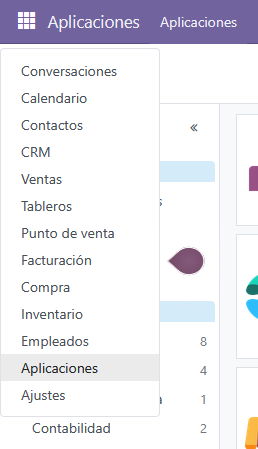
\includegraphics[width=0.5\textwidth]{pr2odoo01-modulosInstalados.png}
    \caption{Modulos instalados}
\end{figure}
\FloatBarrier

\section{Análisis de módulos}

\subsection{Facturación}
\hyperlink{anchor-indice}{\textbf{Volver}}\\

Permite la creación y gestión de las facturas, controlar sus estados, importar y exportar registros, etc.

\begin{figure}[h!]
    \centering
    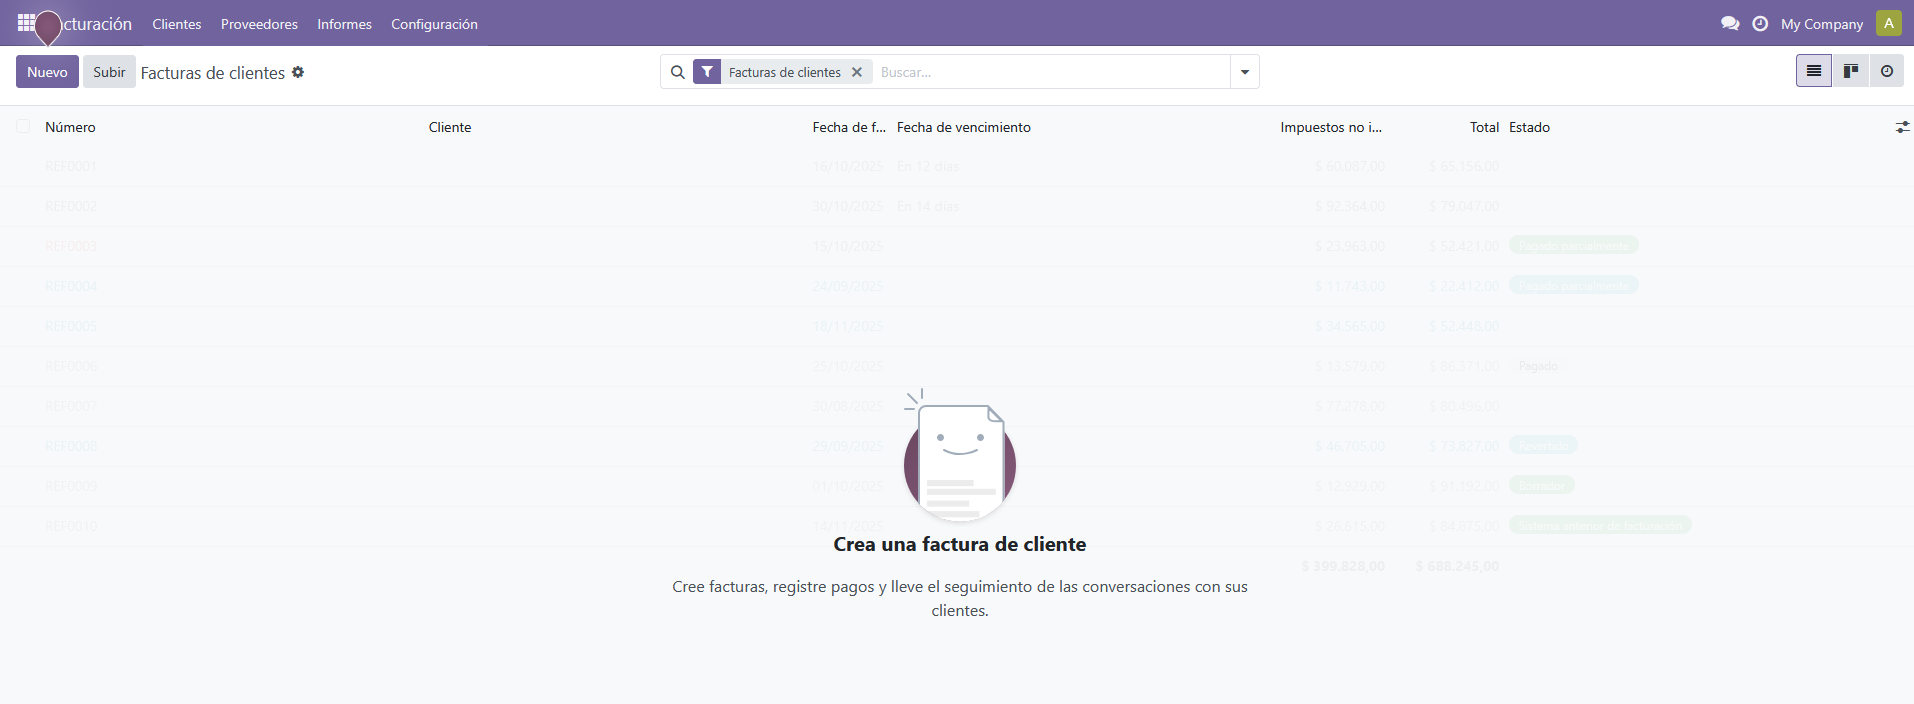
\includegraphics[width=0.5\textwidth]{pr2odoo02-facturacMain.png}
    \caption{Pantalla principal de Facturación}
\end{figure}
\FloatBarrier

Rellenamos los campos con la información pertinente.

\begin{figure}[h!]
    \centering
    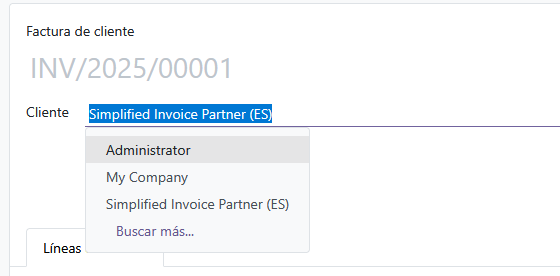
\includegraphics[width=0.5\textwidth]{pr2odoo03-facturac01.png}
    \caption{Cliente}
\end{figure}
\FloatBarrier

\begin{figure}[h!]
    \centering
    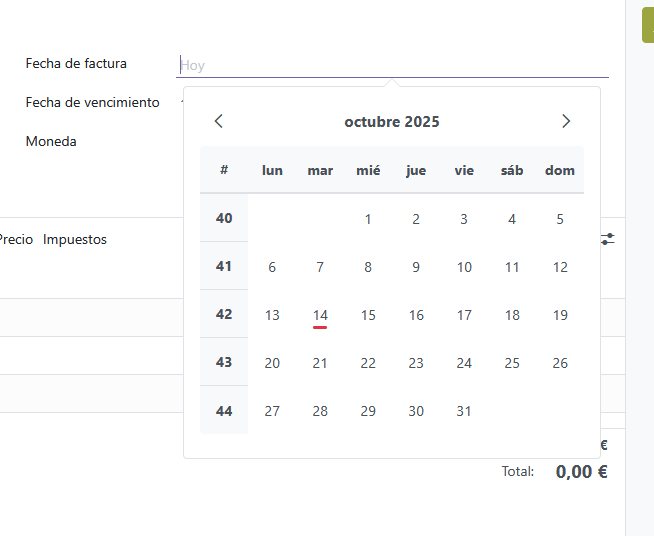
\includegraphics[width=0.5\textwidth]{pr2odoo04-facturac02.png}
    \caption{Fechas de factura}
\end{figure}
\FloatBarrier

\begin{figure}[h!]
    \centering
    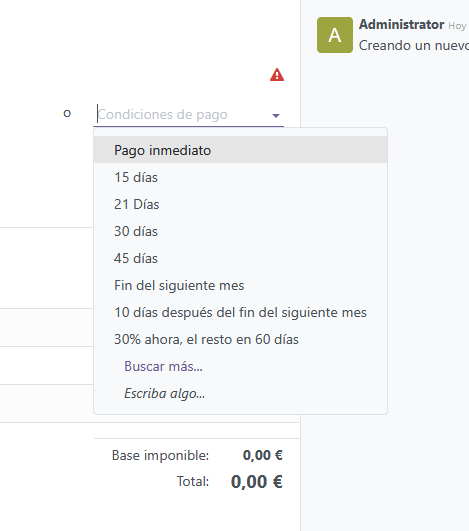
\includegraphics[width=0.5\textwidth]{pr2odoo05-facturac03.png}
    \caption{Condiciones de pago}
\end{figure}
\FloatBarrier

\begin{figure}[h!]
    \centering
    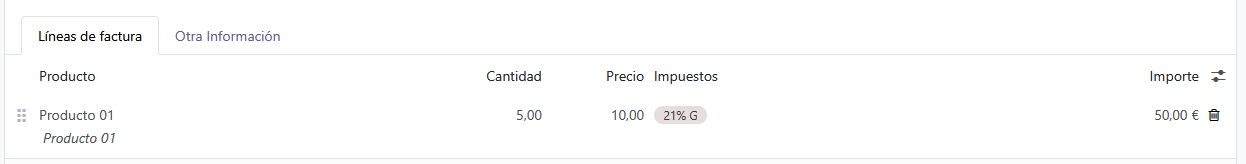
\includegraphics[width=0.5\textwidth]{pr2odoo06-facturac04.png}
    \caption{Productos}
\end{figure}
\FloatBarrier

\begin{figure}[h!]
    \centering
    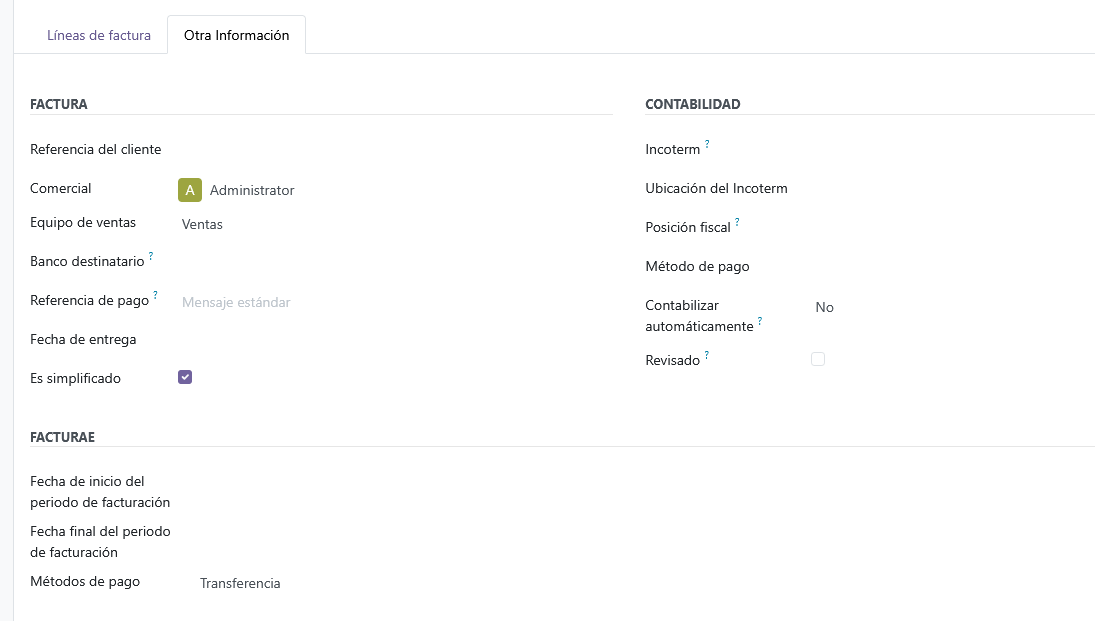
\includegraphics[width=0.5\textwidth]{pr2odoo07-facturac05.png}
    \caption{Otra información}
\end{figure}
\FloatBarrier

\begin{figure}[h!]
    \centering
    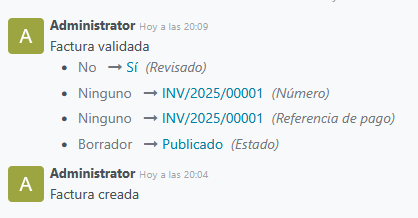
\includegraphics[width=0.5\textwidth]{pr2odoo08-facturac06.png}
    \caption{Resultado tras confirmar factura}
\end{figure}
\FloatBarrier

\begin{figure}[h!]
    \centering
    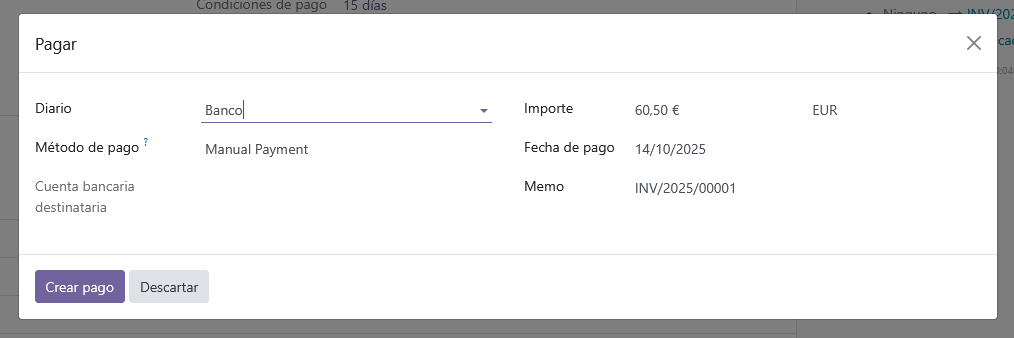
\includegraphics[width=0.5\textwidth]{pr2odoo09-facturac07.png}
    \caption{Pantalla de pago de factura}
\end{figure}
\FloatBarrier

\begin{figure}[h!]
    \centering
    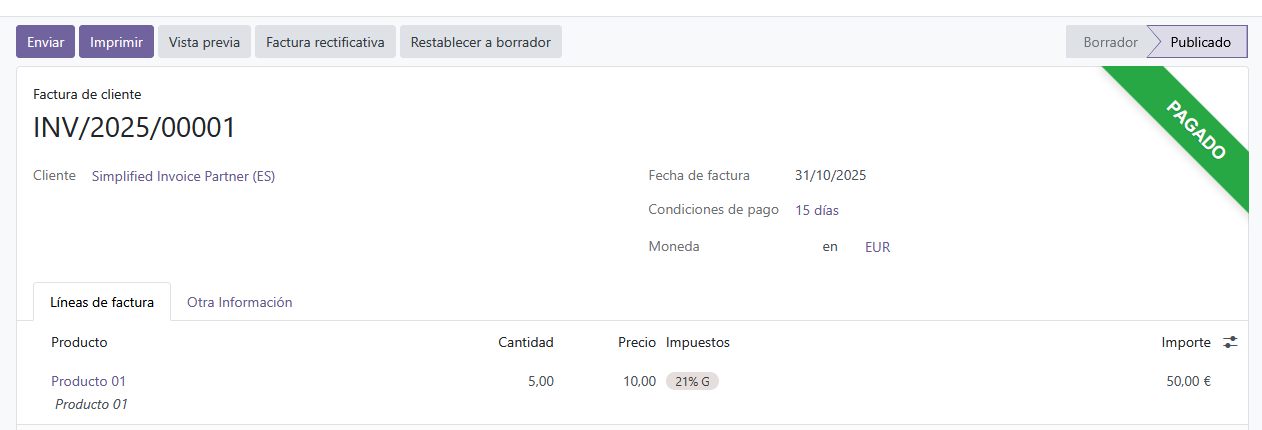
\includegraphics[width=0.5\textwidth]{pr2odoo10-facturac08.png}
    \caption{Factura pagada}
\end{figure}
\FloatBarrier


\subsection{Empleados}
\hyperlink{anchor-indice}{\textbf{Volver}}\\

Aquí podemos crear nuevos empleados, departamentos e informes, así como realizar todos los ajustes necesarios a los mismos. Permite realizar un seguimiento exhaustivo de todos los empleados desde su contratación hasta su terminación si es que esta sucediese, todos sus datos, habilidades, jornada, salidas, entorno de trabajo, etc.


\begin{figure}[h!]
    \centering
    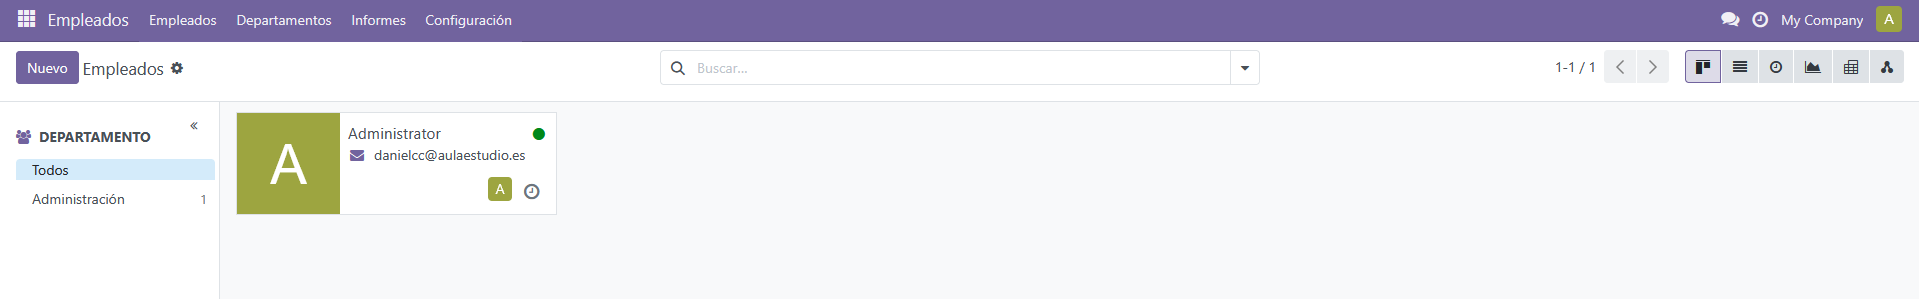
\includegraphics[width=0.5\textwidth]{pr2odoo11-empleadosMain.png}
    \caption{Pantalla principal de Empleados}
\end{figure}
\FloatBarrier

\begin{figure}[h!]
    \centering
    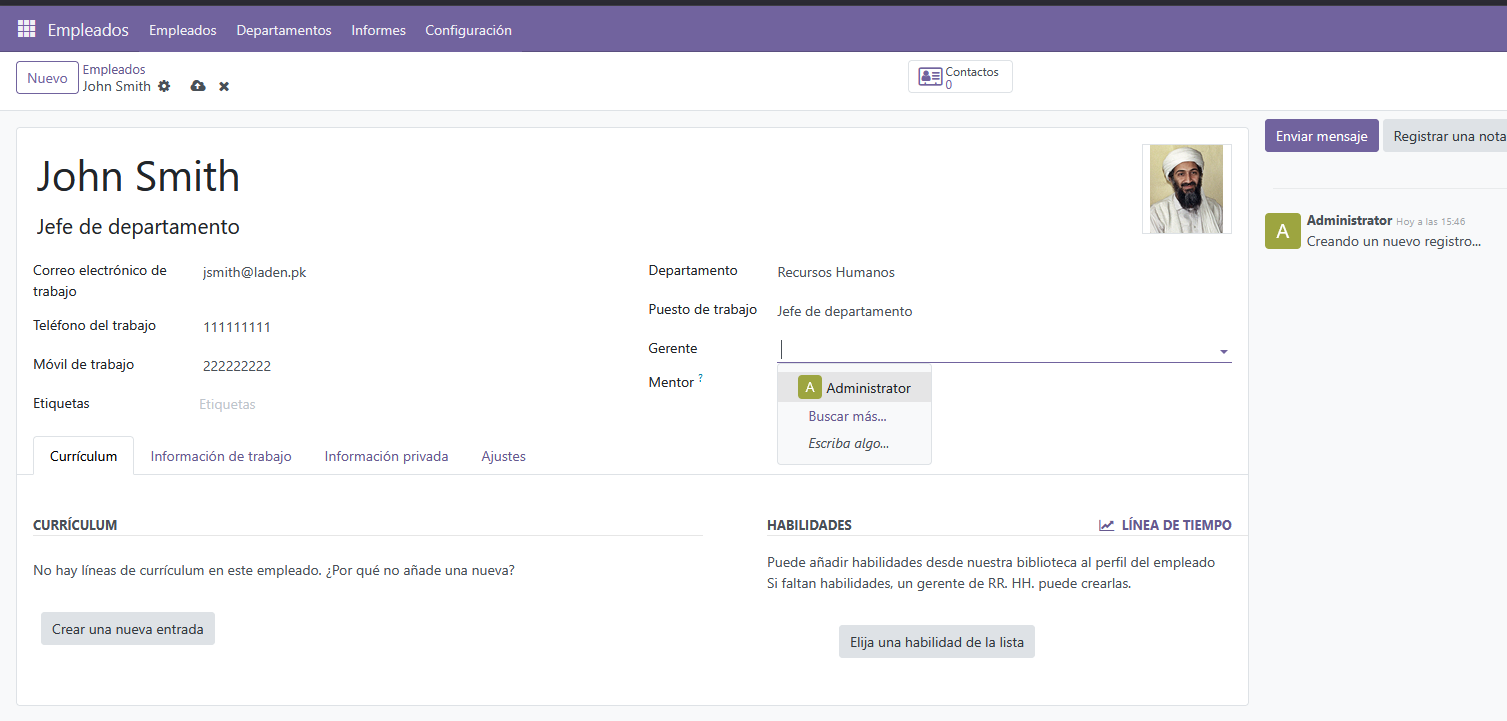
\includegraphics[width=0.5\textwidth]{pr2odoo12-DatosBasicosDeNuevoEmpleado.png}
    \caption{Datos básicos de nuevo empleado}
\end{figure}
\FloatBarrier

\begin{figure}[h!]
    \centering
    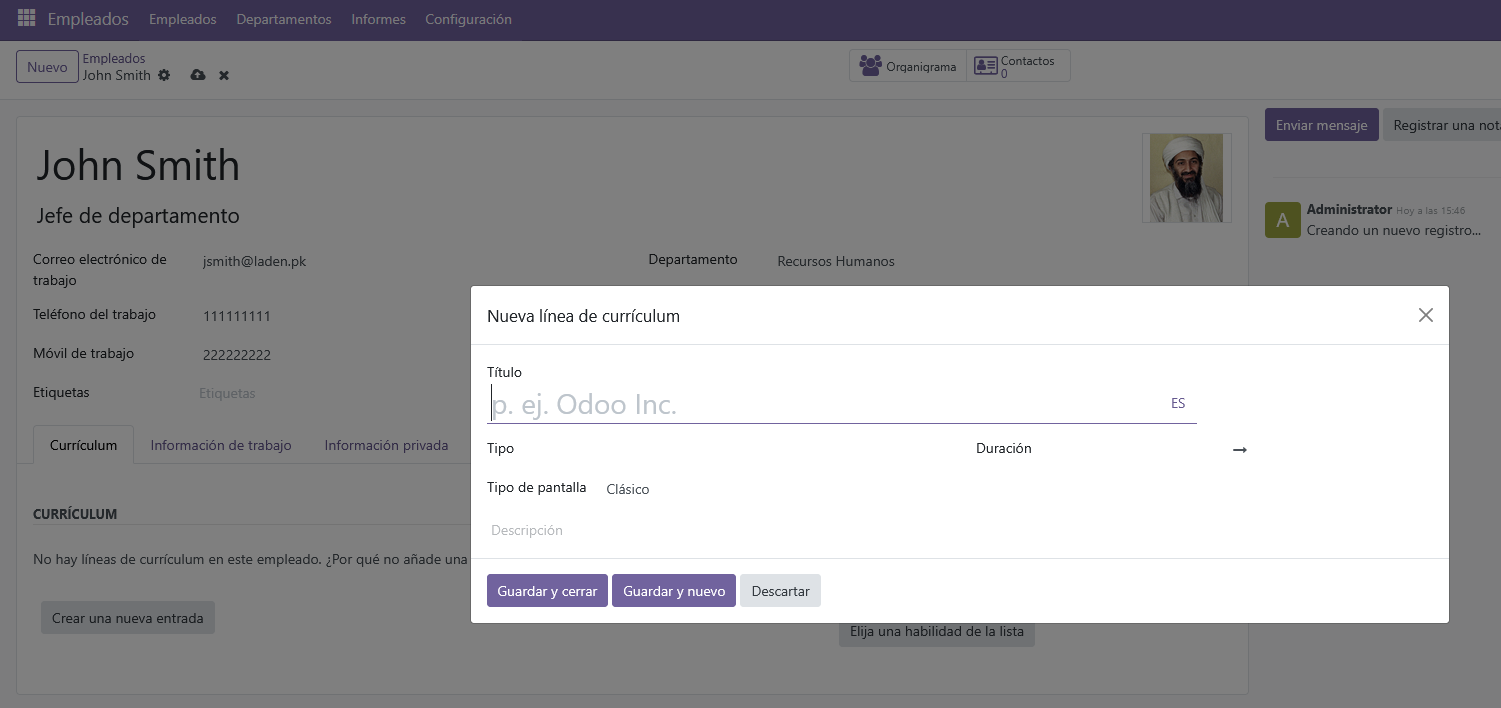
\includegraphics[width=0.5\textwidth]{pr2odoo13-curriculum.png}
    \caption{Curriculum}
\end{figure}
\FloatBarrier

\begin{figure}[h!]
    \centering
    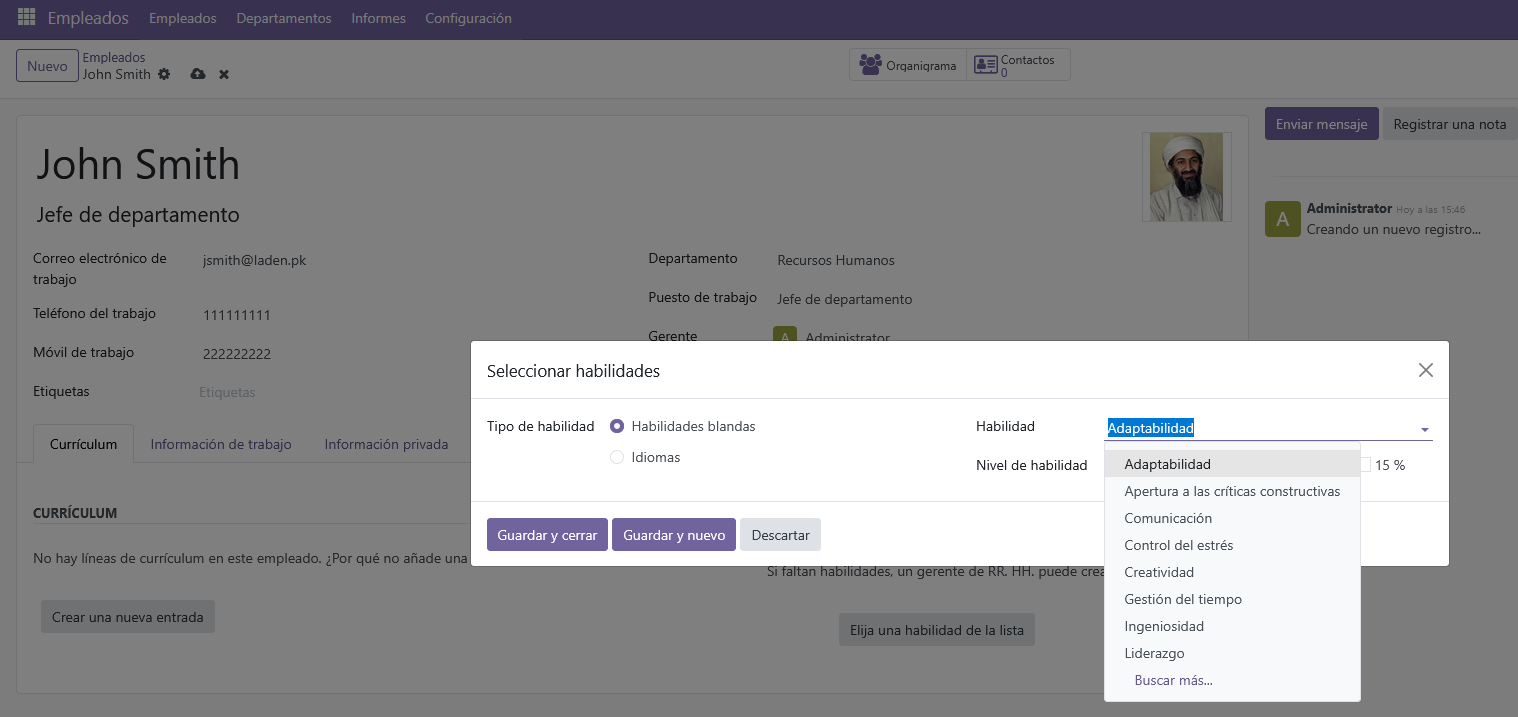
\includegraphics[width=0.5\textwidth]{pr2odoo14-habilidades.png}
    \caption{Habilidades}
\end{figure}
\FloatBarrier

\begin{figure}[h!]
    \centering
    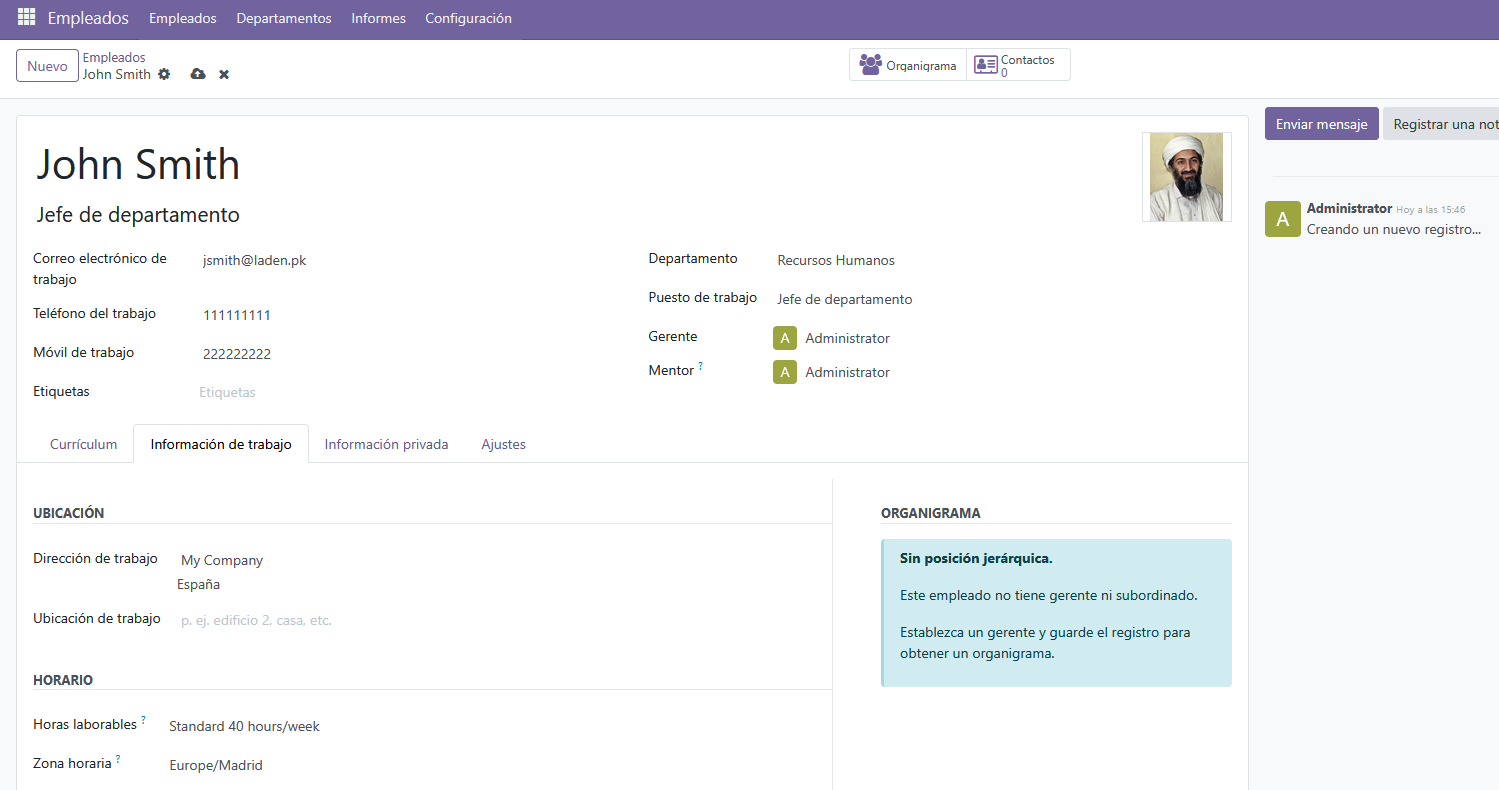
\includegraphics[width=0.5\textwidth]{pr2odoo15-informacionDeTrabajo.png}
    \caption{Información de trabajo}
\end{figure}
\FloatBarrier

\begin{figure}[h!]
    \centering
    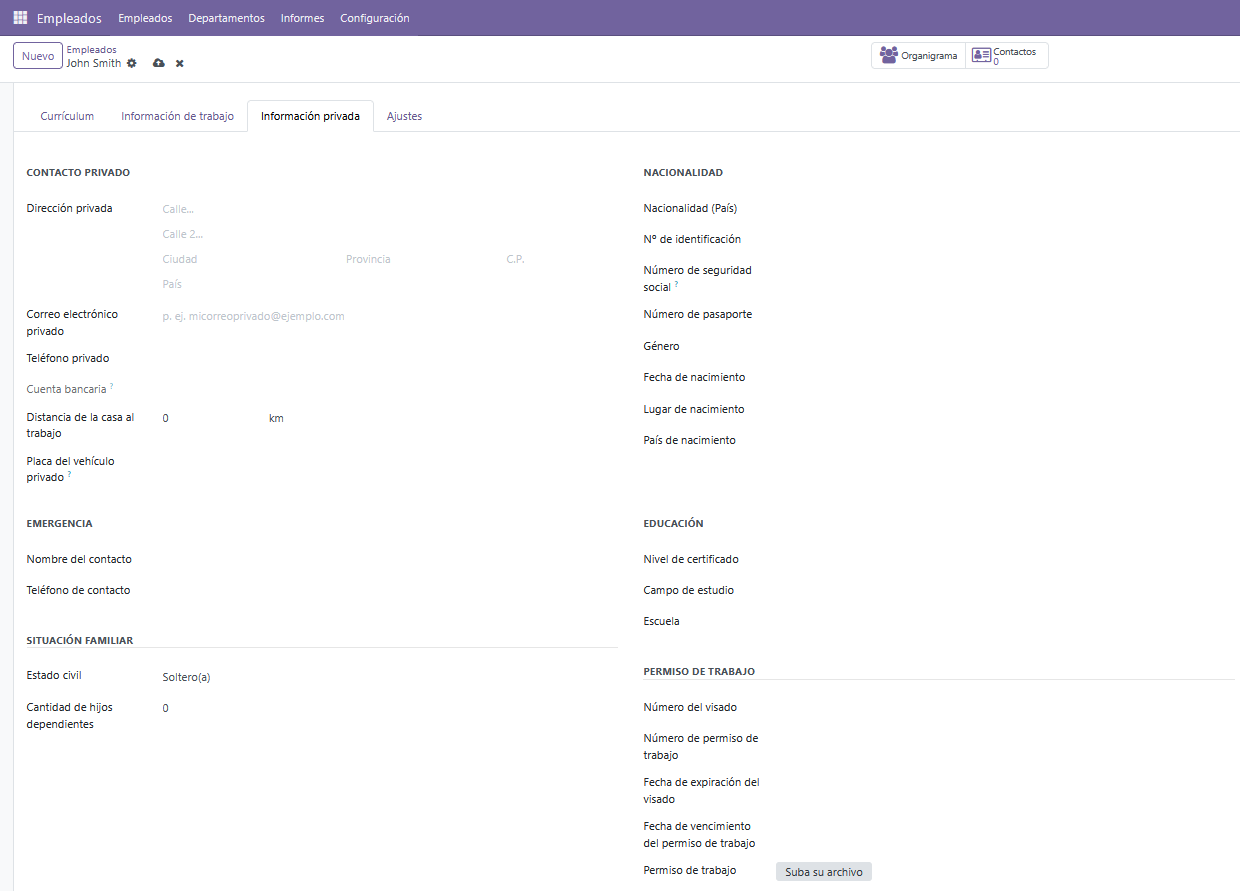
\includegraphics[width=0.5\textwidth]{pr2odoo16-informacionPrivada.png}
    \caption{Información privada}
\end{figure}
\FloatBarrier

\begin{figure}[h!]
    \centering
    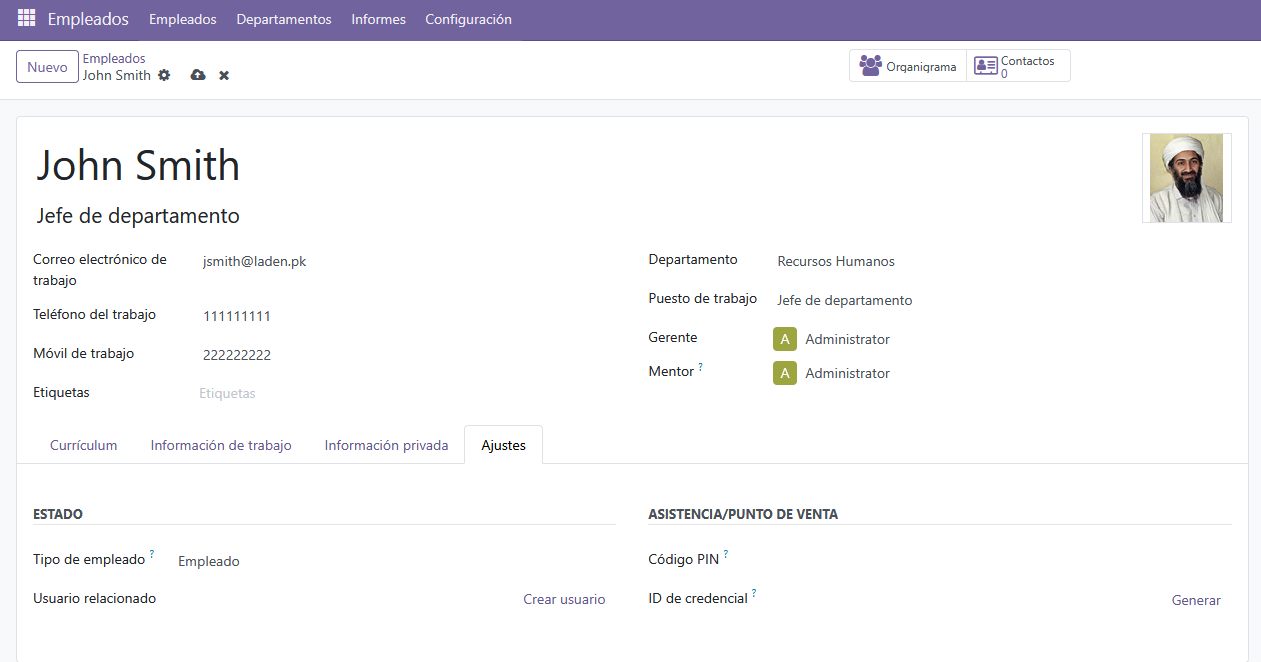
\includegraphics[width=0.5\textwidth]{pr2odoo17-ajustes.png}
    \caption{Ajustes}
\end{figure}
\FloatBarrier

\begin{figure}[h!]
    \centering
    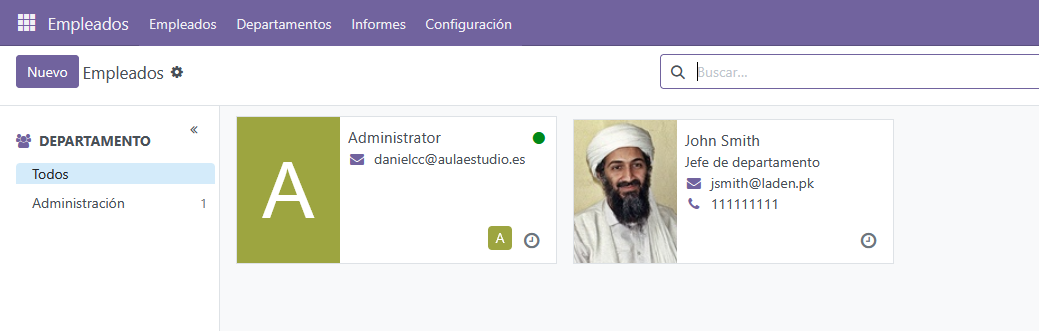
\includegraphics[width=0.5\textwidth]{pr2odoo18-empleadoCreado.png}
    \caption{Empleado creado}
\end{figure}
\FloatBarrier

\begin{figure}[h!]
    \centering
    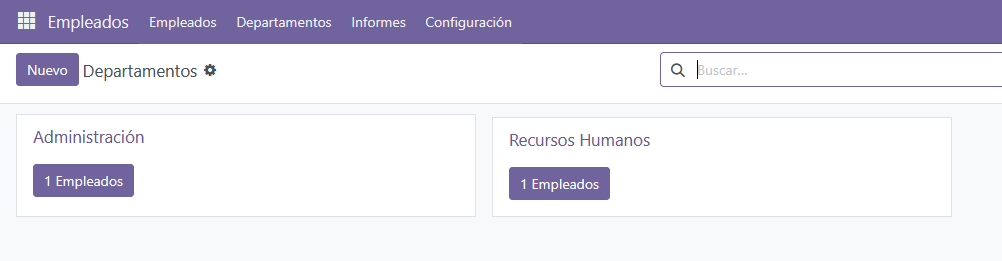
\includegraphics[width=0.5\textwidth]{pr2odoo19-departamentos.png}
    \caption{Departamentos actuales}
\end{figure}
\FloatBarrier

\begin{figure}[h!]
    \centering
    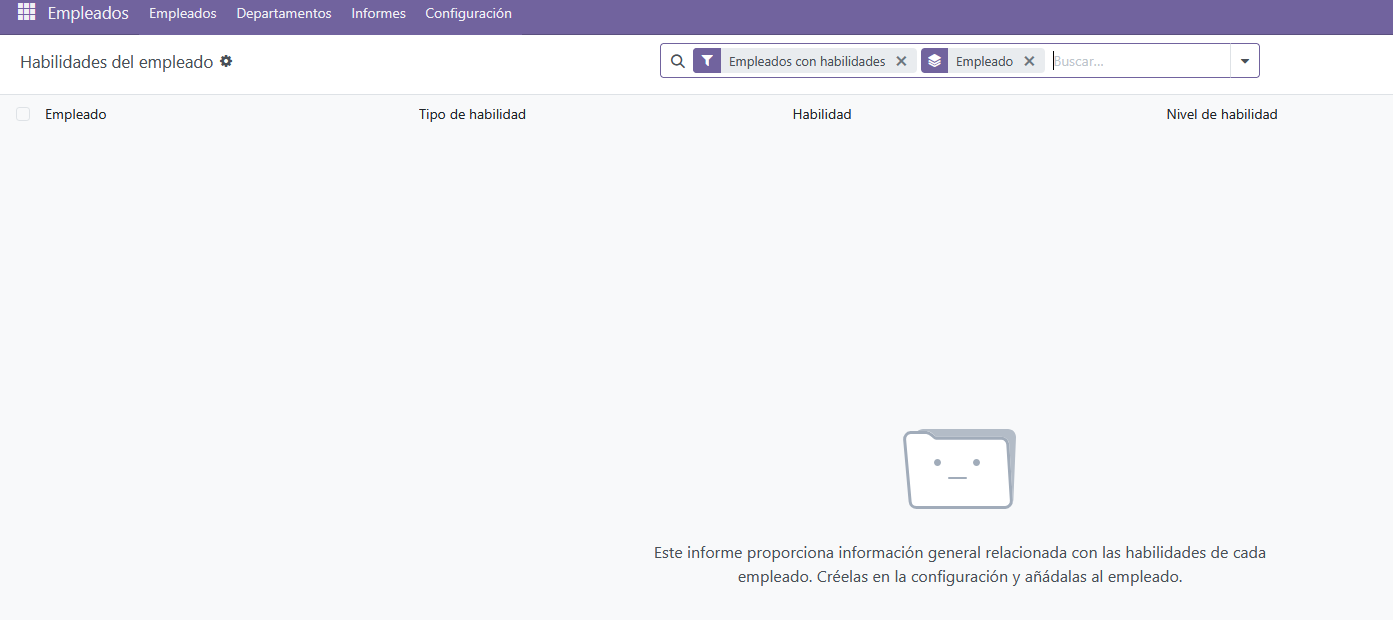
\includegraphics[width=0.5\textwidth]{pr2odoo20-habilidadesDeEmpleado.png}
    \caption{Habilidades de empleado}
\end{figure}
\FloatBarrier

\begin{figure}[h!]
    \centering
    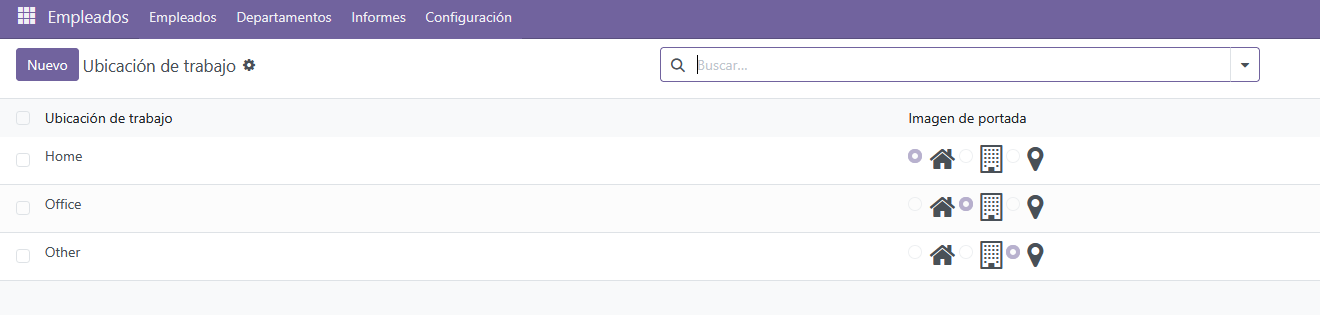
\includegraphics[width=0.5\textwidth]{pr2odoo21-ubicacionDeTrabajo.png}
    \caption{Ubicación de trabajo}
\end{figure}
\FloatBarrier

\begin{figure}[h!]
    \centering
    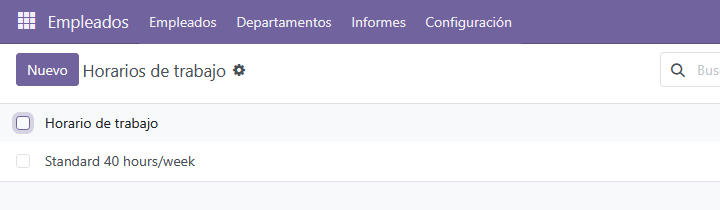
\includegraphics[width=0.5\textwidth]{pr2odoo22-horarios.png}
    \caption{Horarios de trabajo}
\end{figure}
\FloatBarrier

\begin{figure}[h!]
    \centering
    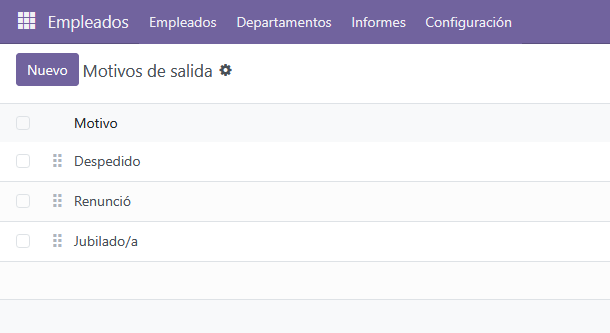
\includegraphics[width=0.5\textwidth]{pr2odoo23-motivosSalida.png}
    \caption{Motivos de salida}
\end{figure}
\FloatBarrier

\begin{figure}[h!]
    \centering
    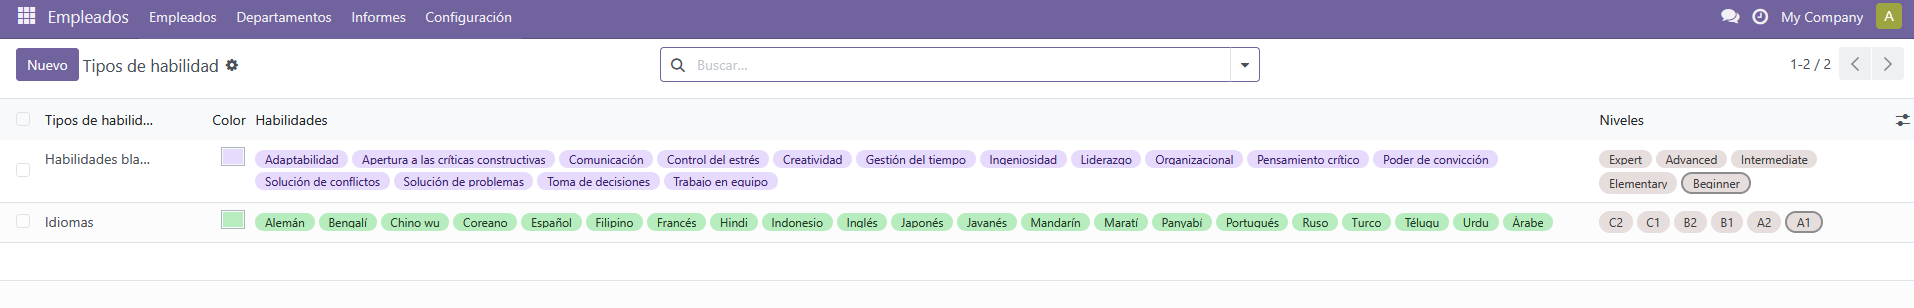
\includegraphics[width=0.5\textwidth]{pr2odoo24-tiposHabilidad.png}
    \caption{Tipos de habilidad}
\end{figure}
\FloatBarrier

\begin{figure}[h!]
    \centering
    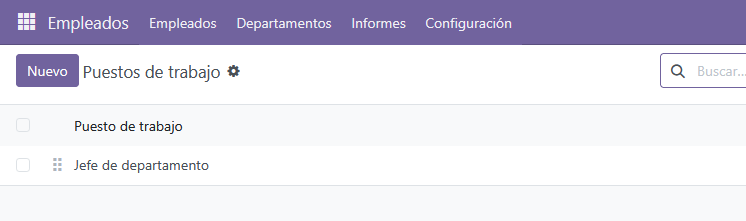
\includegraphics[width=0.5\textwidth]{pr2odoo25-puestosTrabajo.png}
    \caption{Puestos de trabajo}
\end{figure}
\FloatBarrier

\begin{figure}[h!]
    \centering
    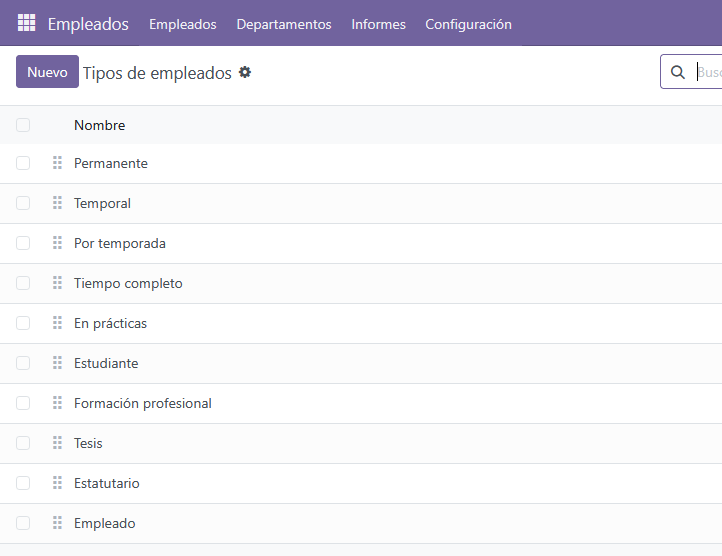
\includegraphics[width=0.5\textwidth]{pr2odoo26-tiposEmpleado.png}
    \caption{Tipos de empleado}
\end{figure}
\FloatBarrier


\subsection{Compras}
\hyperlink{anchor-indice}{\textbf{Volver}}\\

Este módulo se ocupa del proceso de compras, creación de presupuesto, seguimiento de recepción de productos y pagos según acordado, categorización de facturas según estado actual, informes de análisis de las compras realizadas o en curso, listas de precios y proveedores, etc.

Los presupuestos y consecuentes facturas tienen absolutamente todos los detalles y requisitos en cuenta, desde los métodos y tipos de pago hasta el modelo de recepción de productos.

\begin{figure}[h!]
    \centering
    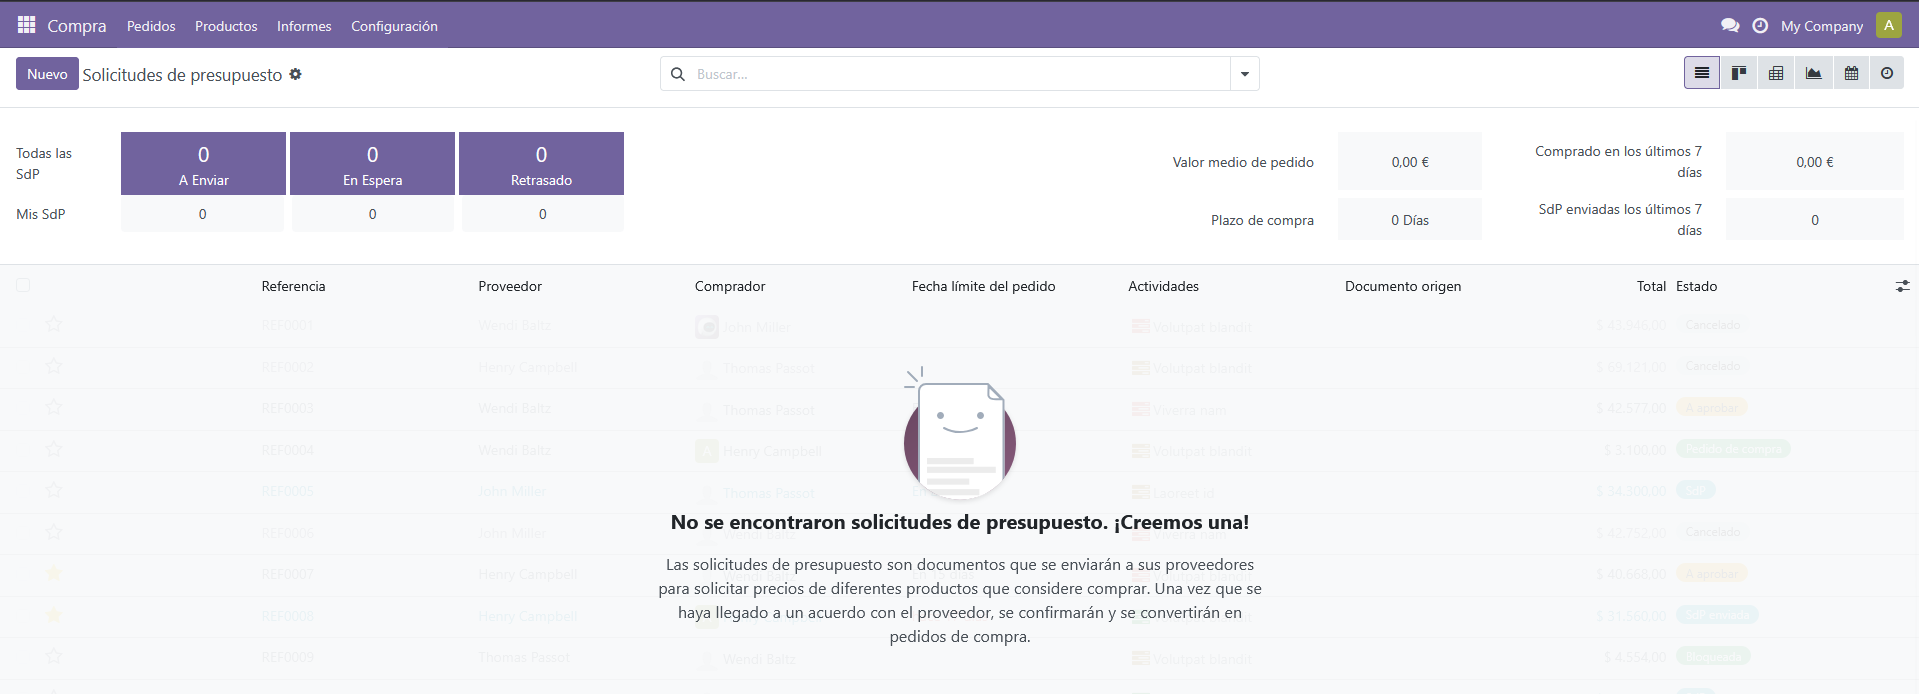
\includegraphics[width=0.5\textwidth]{pr2odoo27-pantallaPrincipalCompras.png}
    \caption{Pantalla principal de compras}
\end{figure}
\FloatBarrier

\begin{figure}[h!]
    \centering
    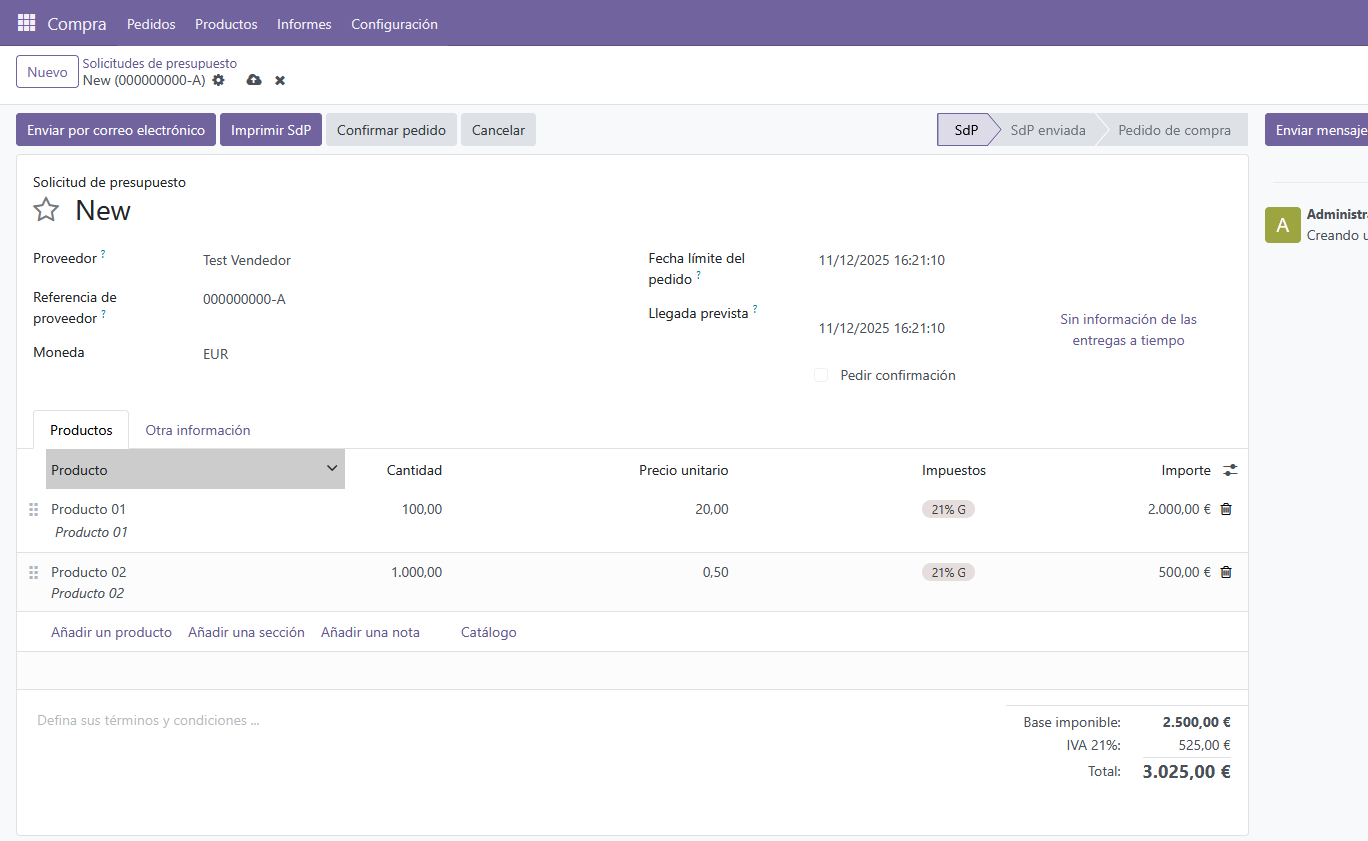
\includegraphics[width=0.5\textwidth]{pr2odoo28-nuevoPresupuesto.png}
    \caption{Nuevo presupuesto: información básica y productos}
\end{figure}
\FloatBarrier

\begin{figure}[h!]
    \centering
    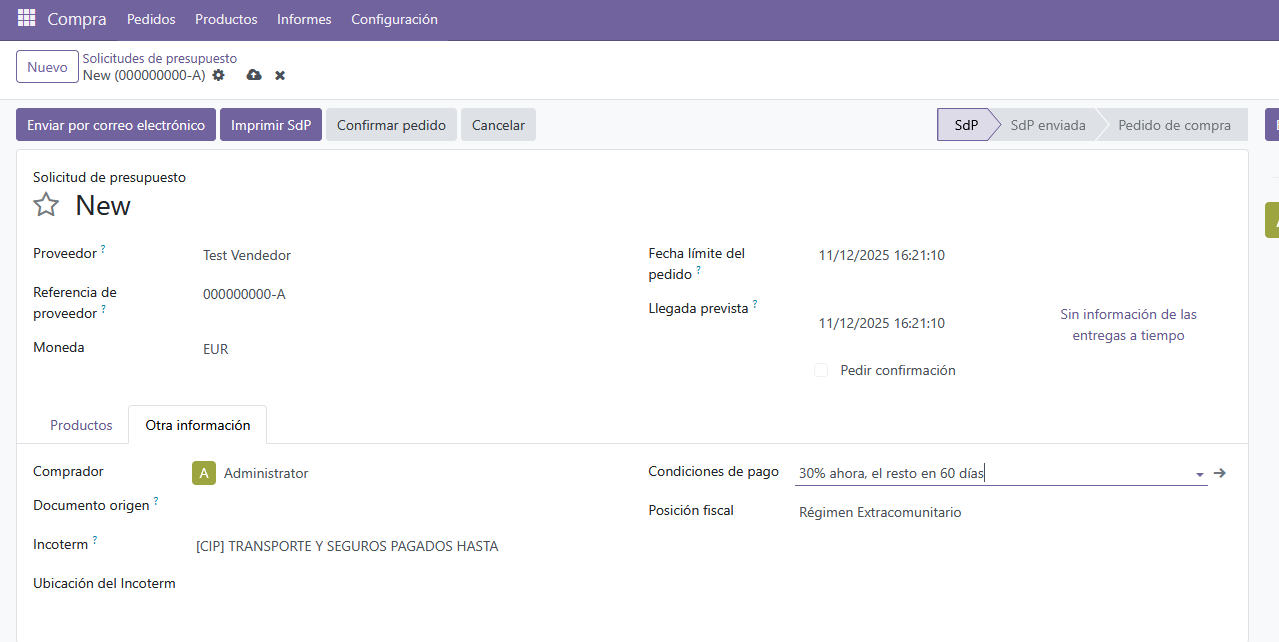
\includegraphics[width=0.5\textwidth]{pr2odoo29-otraInfo.png}
    \caption{Otra información}
\end{figure}
\FloatBarrier

\begin{figure}[h!]
    \centering
    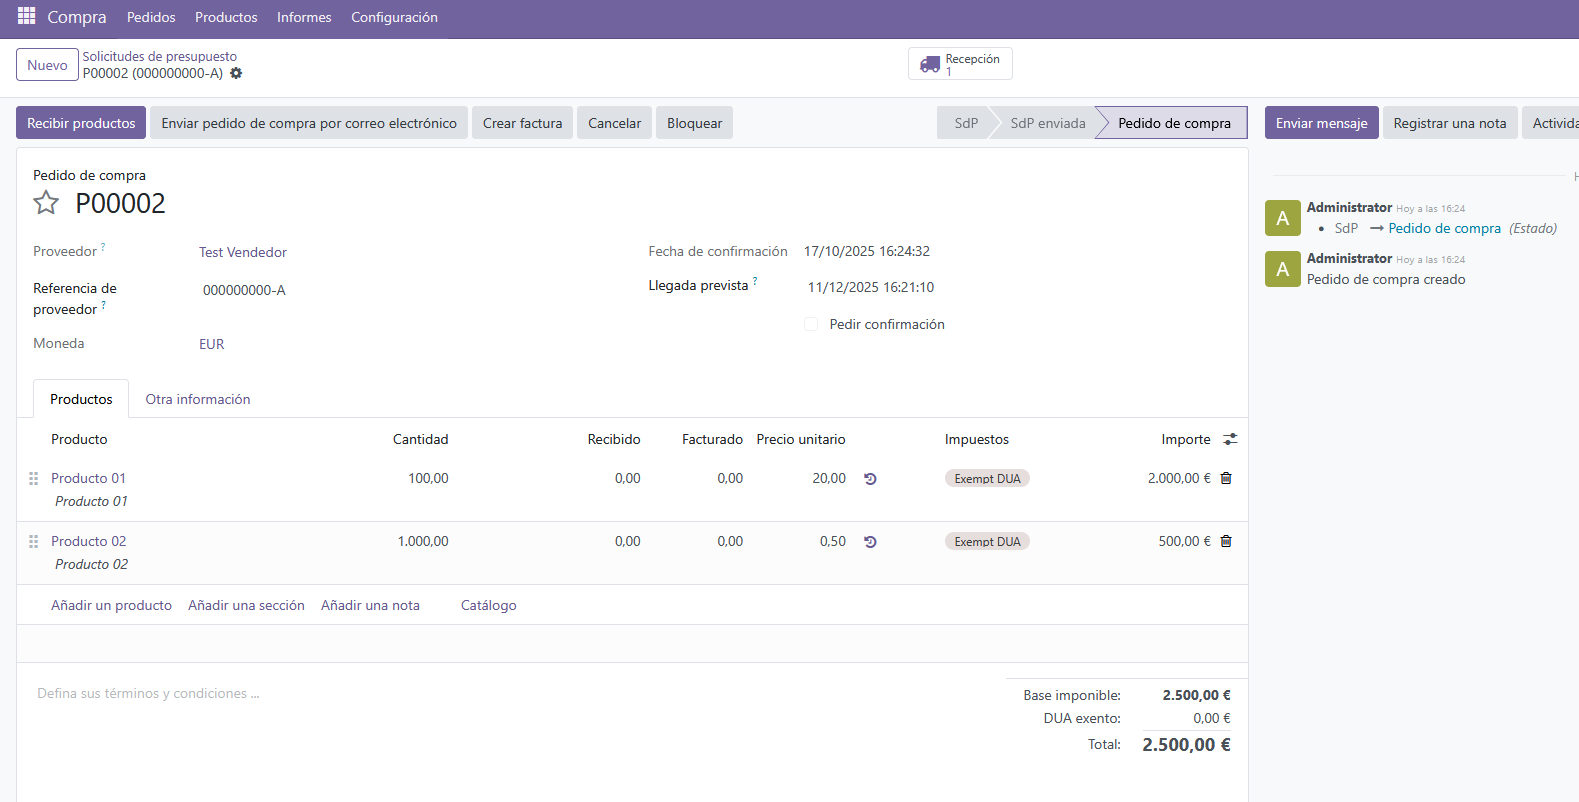
\includegraphics[width=0.5\textwidth]{pr2odoo30-pedidoCreado.png}
    \caption{Pedido creado}
\end{figure}
\FloatBarrier

\begin{figure}[h!]
    \centering
    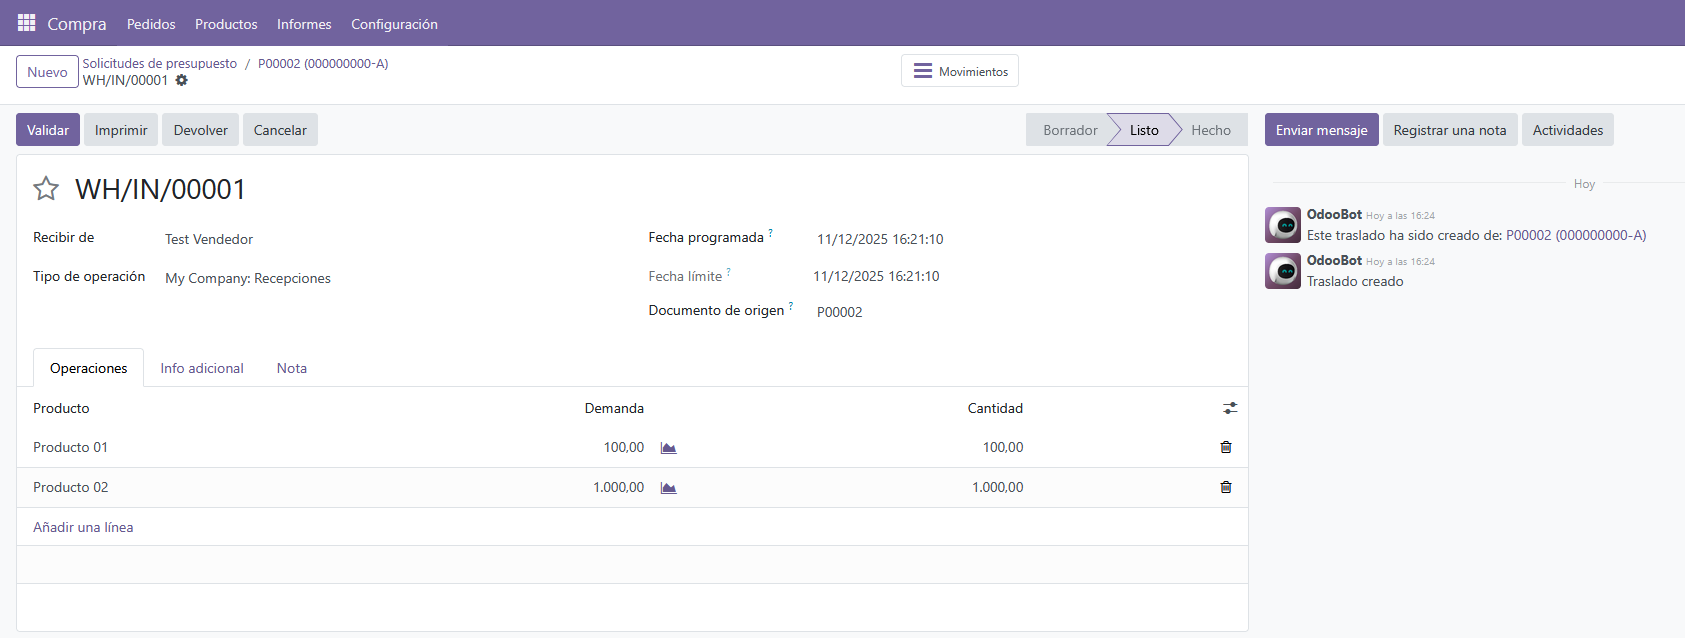
\includegraphics[width=0.5\textwidth]{pr2odoo31-productosRecibidos.png}
    \caption{Productos recibidos}
\end{figure}
\FloatBarrier

\begin{figure}[h!]
    \centering
    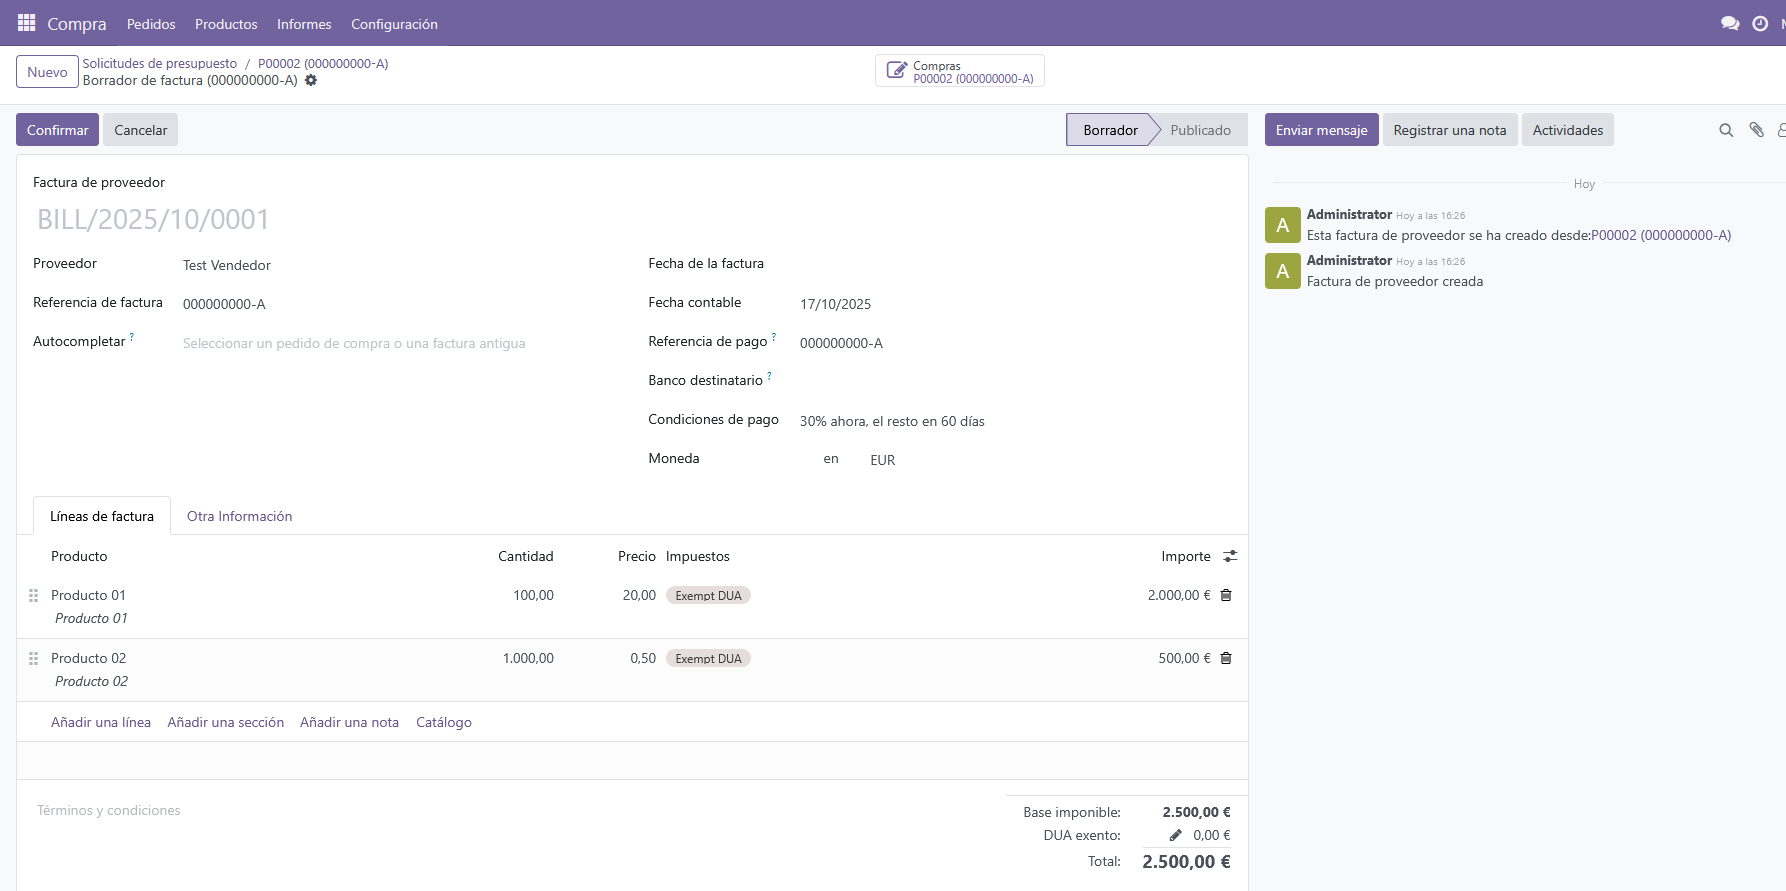
\includegraphics[width=0.5\textwidth]{pr2odoo32-facturaProveedorCreada.png}
    \caption{Factura de proveedor creada}
\end{figure}
\FloatBarrier

\begin{figure}[h!]
    \centering
    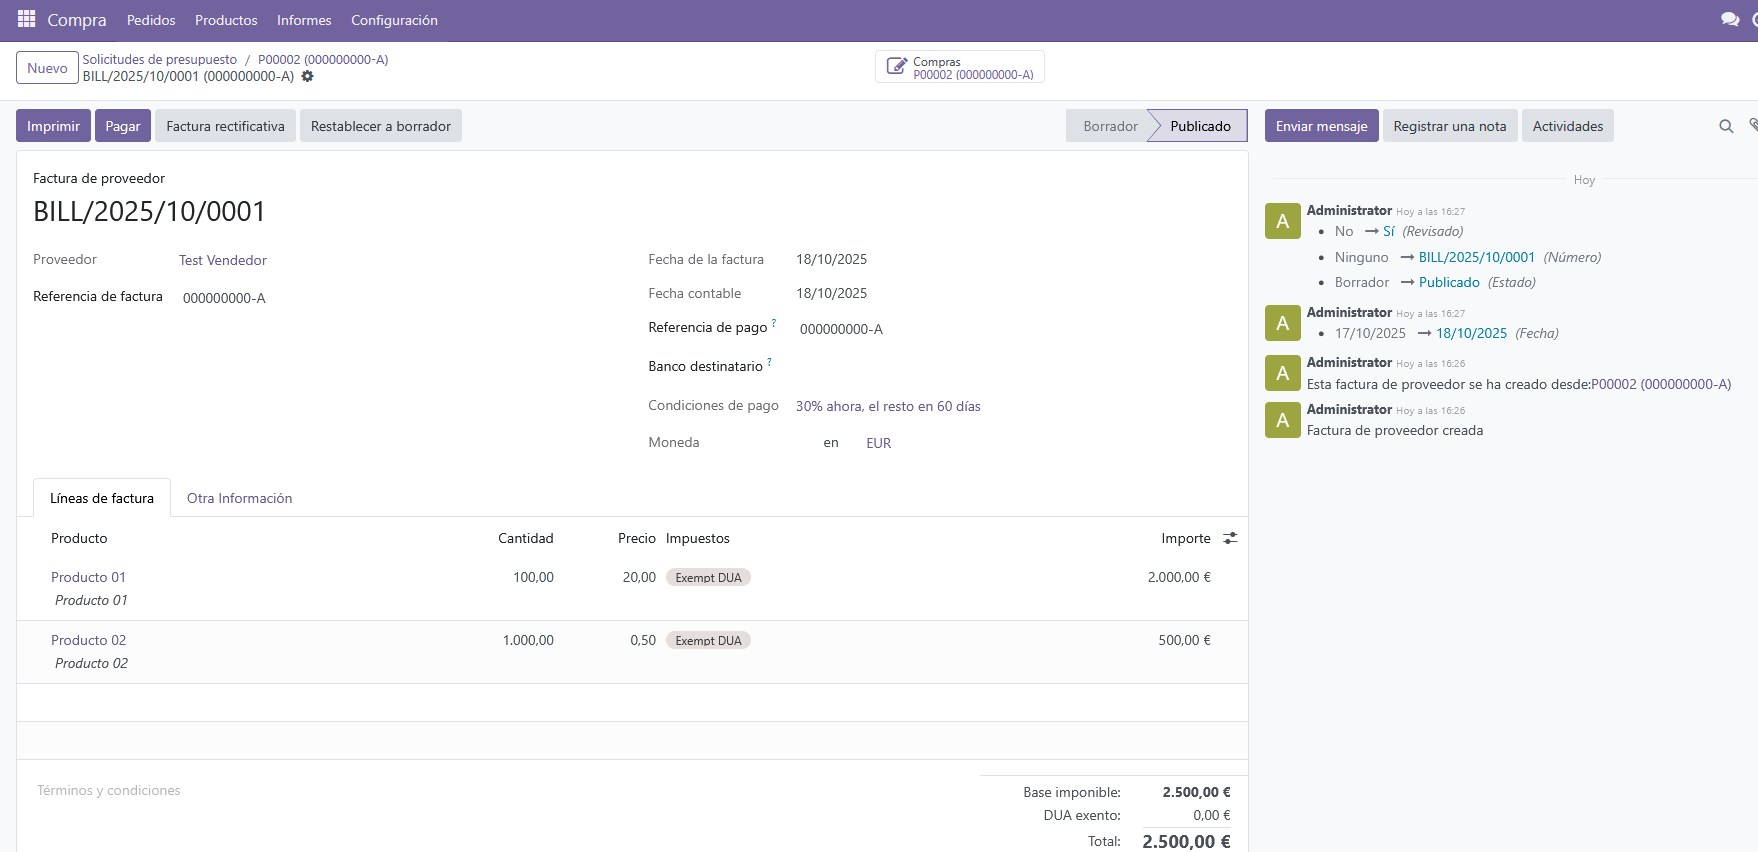
\includegraphics[width=0.5\textwidth]{pr2odoo33-preparadaParaPago.png}
    \caption{Factura preparada para pago}
\end{figure}
\FloatBarrier

\begin{figure}[h!]
    \centering
    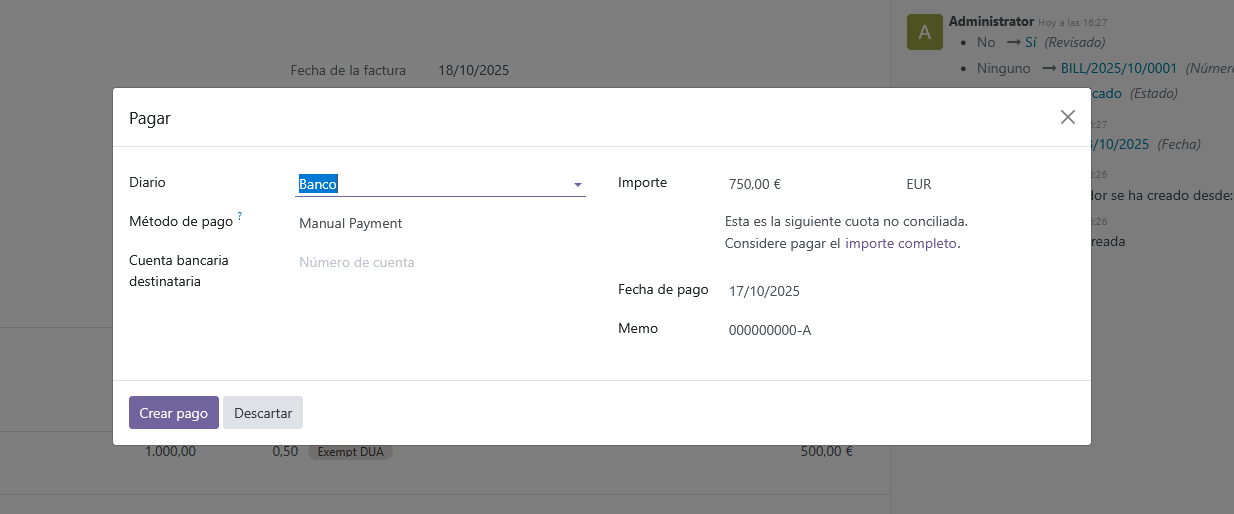
\includegraphics[width=0.5\textwidth]{pr2odoo34-pantallaPago.png}
    \caption{Pantalla de pago}
\end{figure}
\FloatBarrier

\begin{figure}[h!]
    \centering
    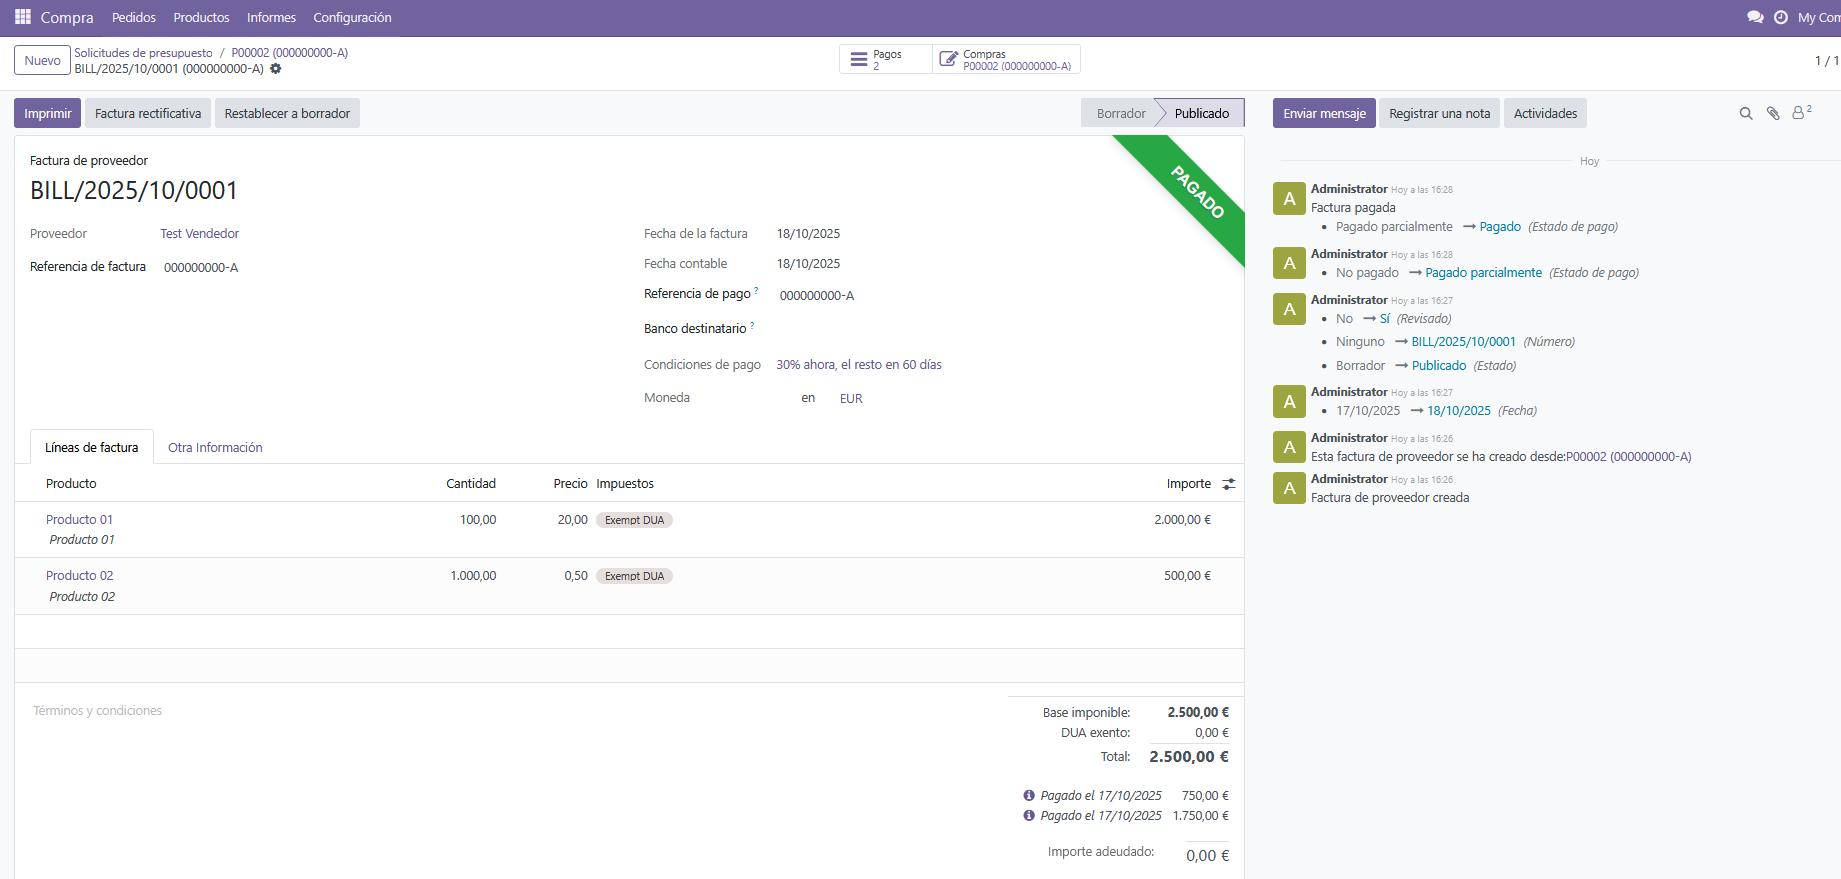
\includegraphics[width=0.5\textwidth]{pr2odoo35-facturaPagada.png}
    \caption{Factura pagada}
\end{figure}
\FloatBarrier

\begin{figure}[h!]
    \centering
    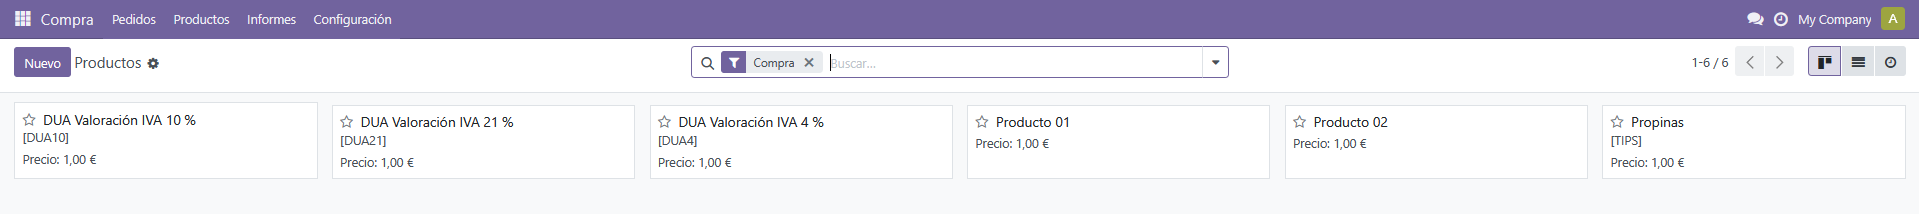
\includegraphics[width=0.5\textwidth]{pr2odoo36-pantallaProductos.png}
    \caption{Pantalla de productos}
\end{figure}
\FloatBarrier

\begin{figure}[h!]
    \centering
    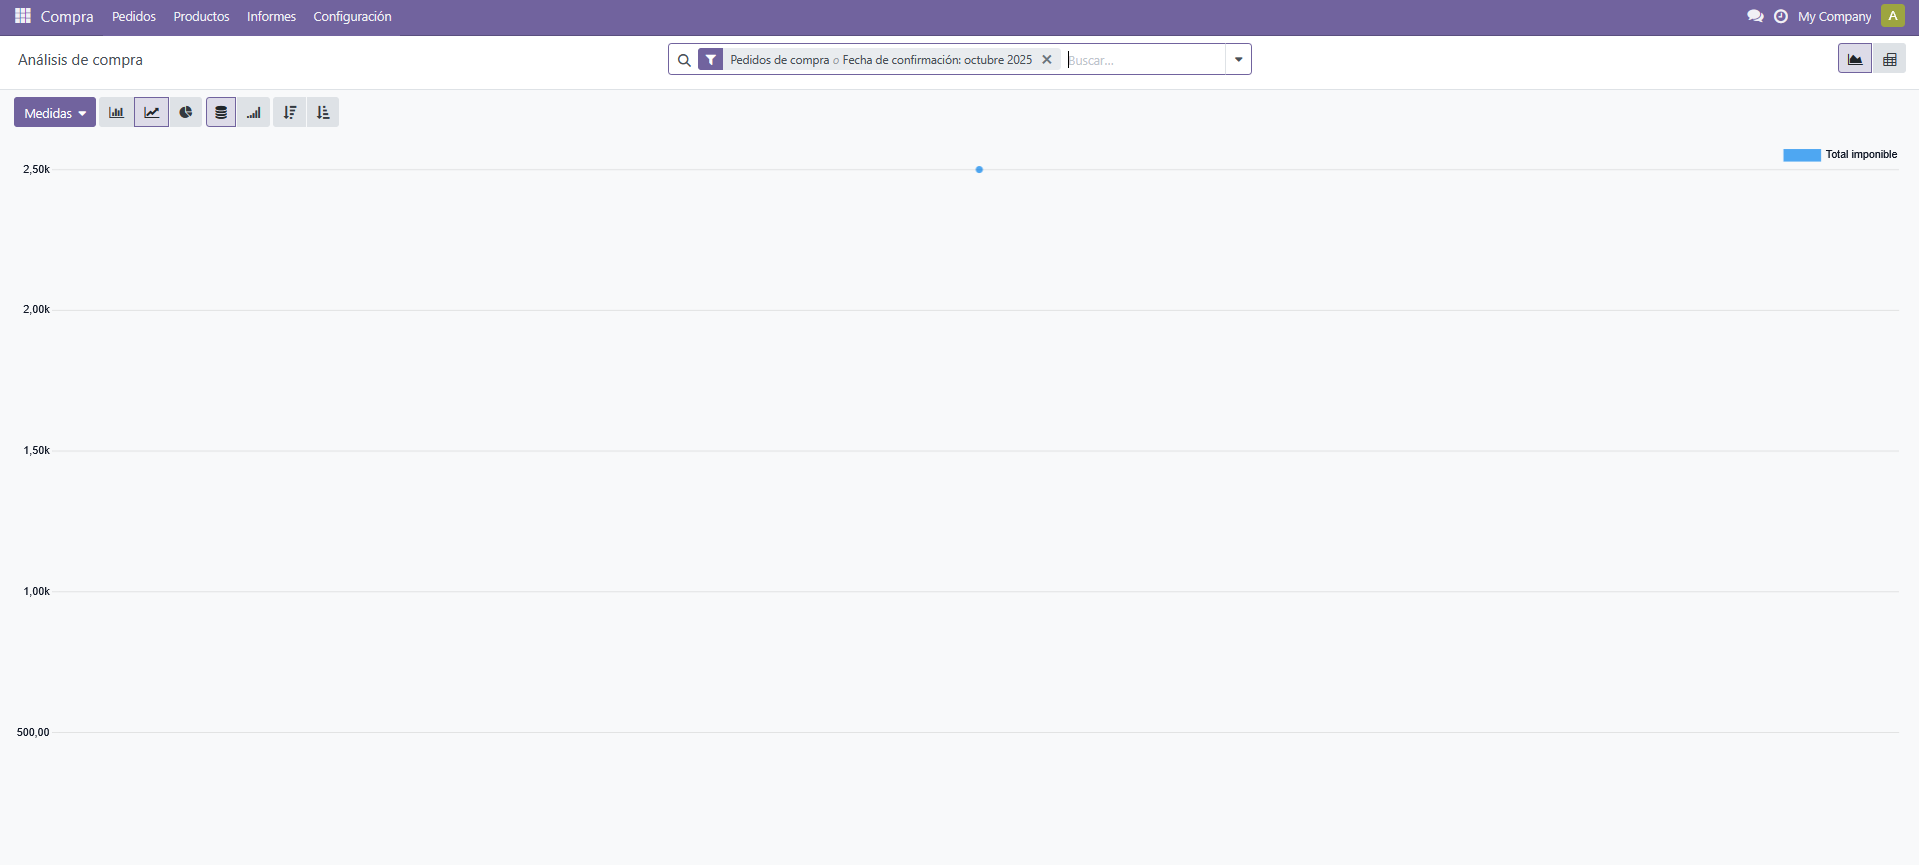
\includegraphics[width=0.5\textwidth]{pr2odoo37-analisisCompras.png}
    \caption{Pantalla de informes de análisis de compras}
\end{figure}
\FloatBarrier

\begin{figure}[h!]
    \centering
    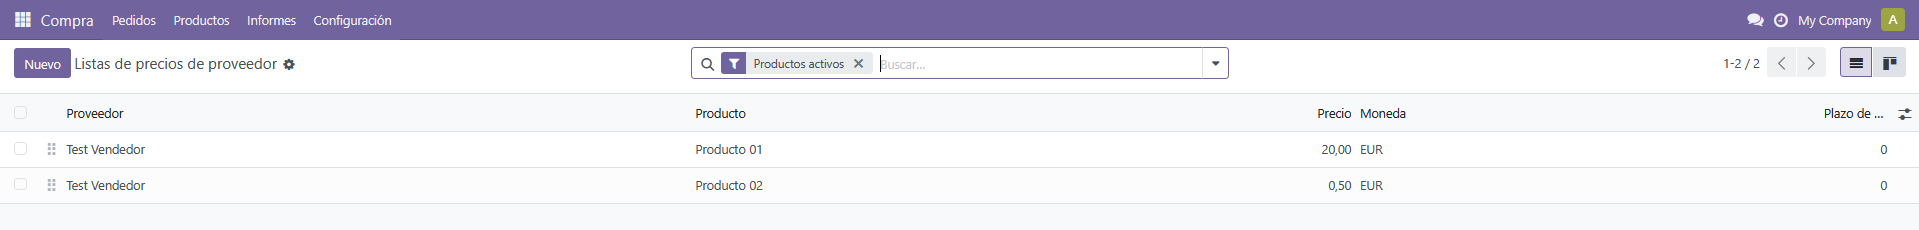
\includegraphics[width=0.5\textwidth]{pr2odoo38-preciosProveedor.png}
    \caption{Lista de precios de proveedores}
\end{figure}
\FloatBarrier

\begin{figure}[h!]
    \centering
    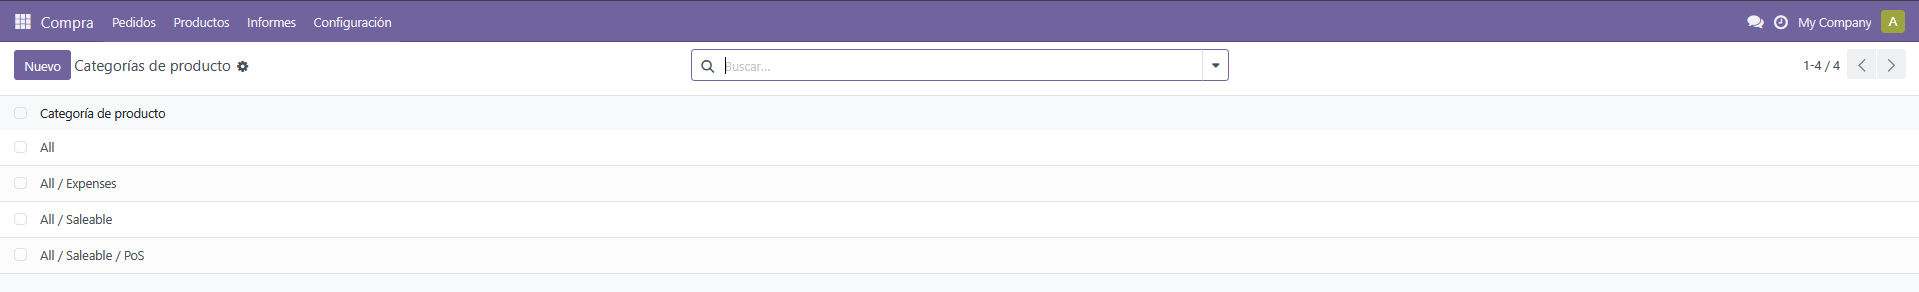
\includegraphics[width=0.5\textwidth]{pr2odoo39-categoriasPrioductos.png}
    \caption{Categorías de productos}
\end{figure}
\FloatBarrier


\subsection{Ventas}
\hyperlink{anchor-indice}{\textbf{Volver}}\\

Módulo muy parecido a compras, aplicado a las ventas. De igual forma cubre todos los aspectos del proceso, con seguimiento de todos los elementos del proceso: presupuestos, pedidos, equipos de ventas y clientes.

Distingue también las secciones para pedidos a facturar y para ventas adicionales, informes de ventas, comerciales, de productos y de clientes, así como tambén permite configurar todos los aspectos necesarios en:
\begin{itemize}
    \item Pedidos:
    \begin{enumerate}
        \item Encabezados.
        \item Etiquetas.
    \end{enumerate}
    \item Productos:
    \begin{enumerate}
        \item Opciones.
        \item Categorías.
        \item Etiquetas.
    \end{enumerate}
    \item Pagos en línea:
    \begin{enumerate}
        \item Proveedores.
        \item Métodos de pago.
    \end{enumerate}
    \item Planes de actividad.
\end{itemize}

\begin{figure}[h!]
    \centering
    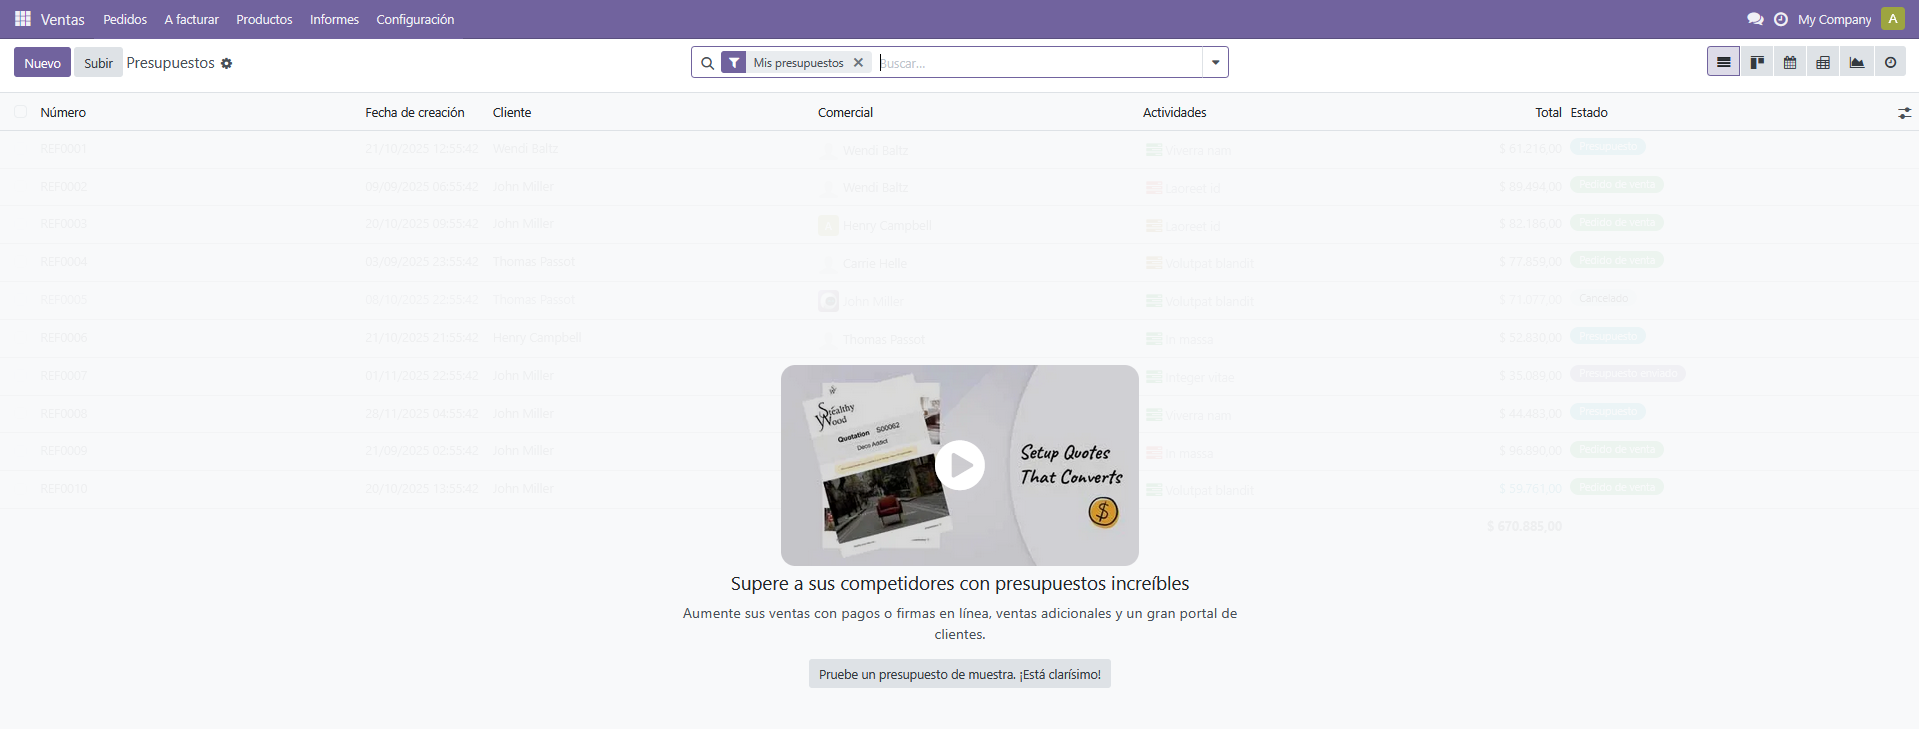
\includegraphics[width=0.5\textwidth]{pr2odoo40-pantallaPrincipalVentas.png}
    \caption{Pantalla principal de ventas}
\end{figure}
\FloatBarrier

\begin{figure}[h!]
    \centering
    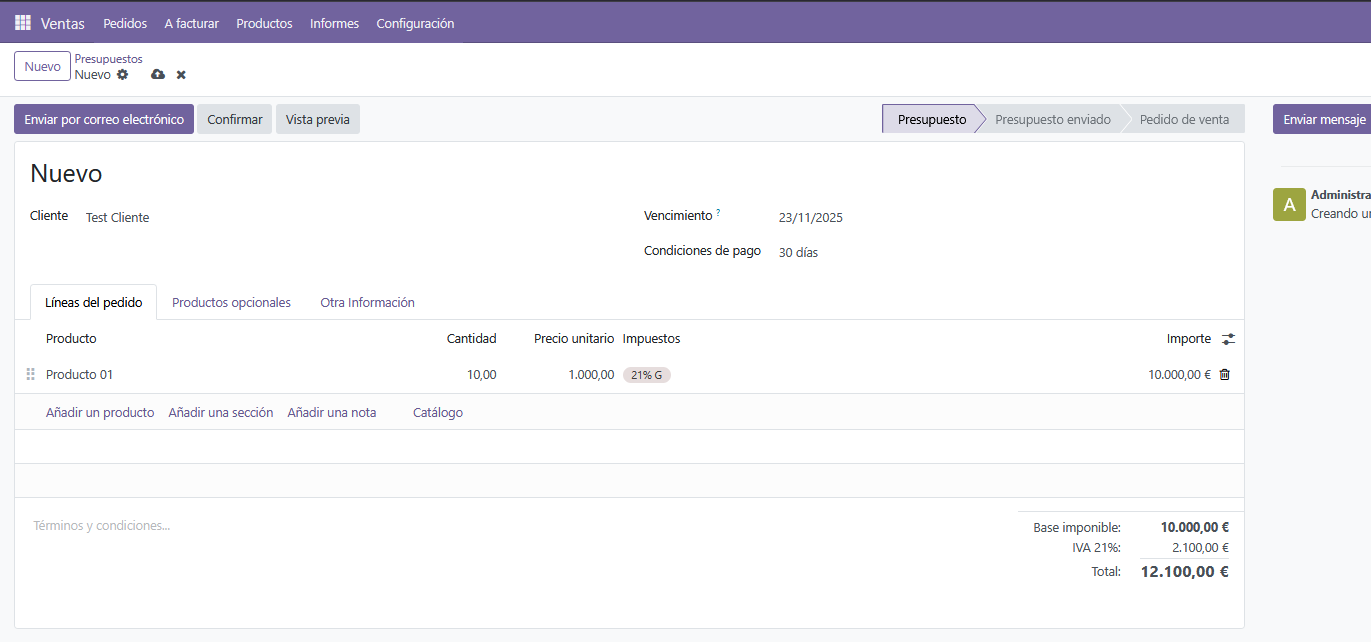
\includegraphics[width=0.5\textwidth]{pr2odoo41-nuevoPresupuesto.png}
    \caption{Nuevo presupuesto de venta}
\end{figure}
\FloatBarrier

\begin{figure}[h!]
    \centering
    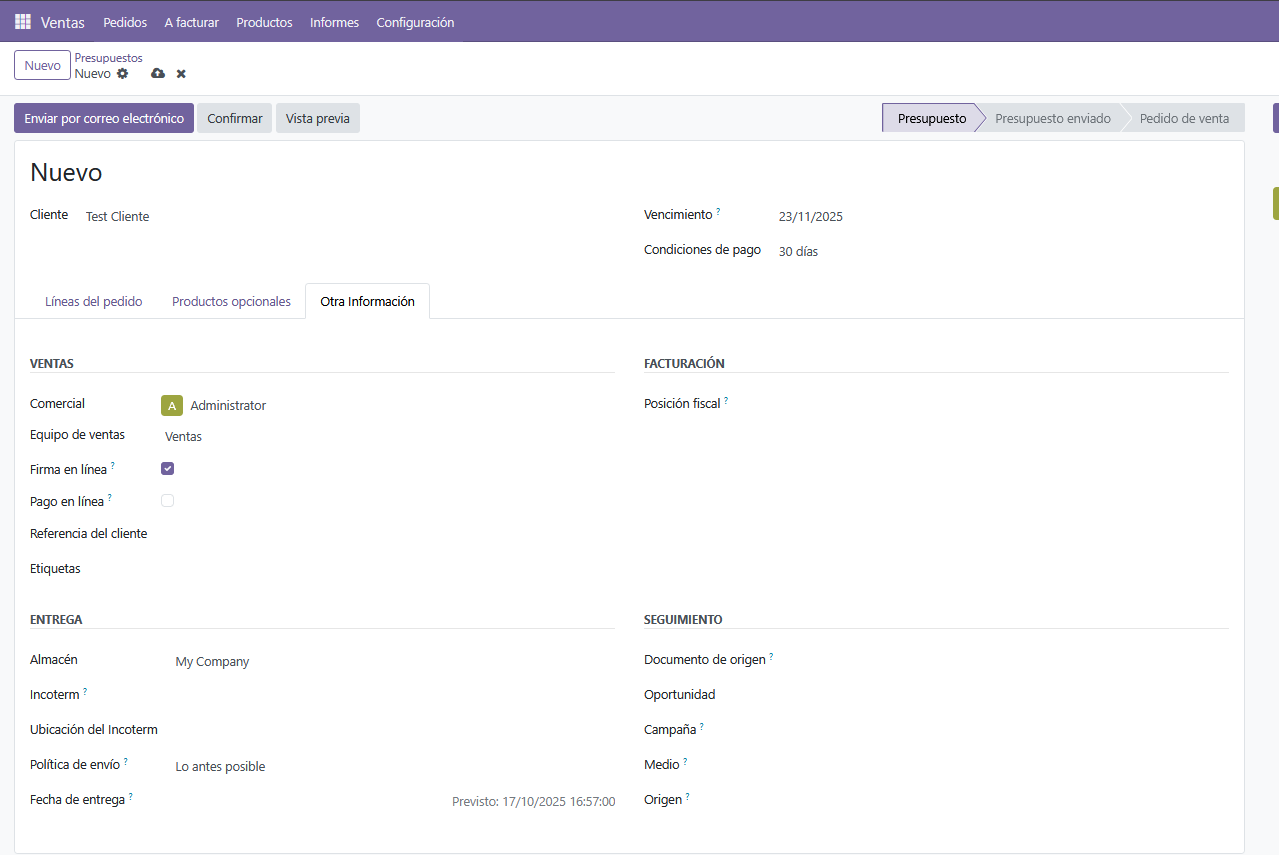
\includegraphics[width=0.5\textwidth]{pr2odoo42-otraInfo.png}
    \caption{Otra información}
\end{figure}
\FloatBarrier

\begin{figure}[h!]
    \centering
    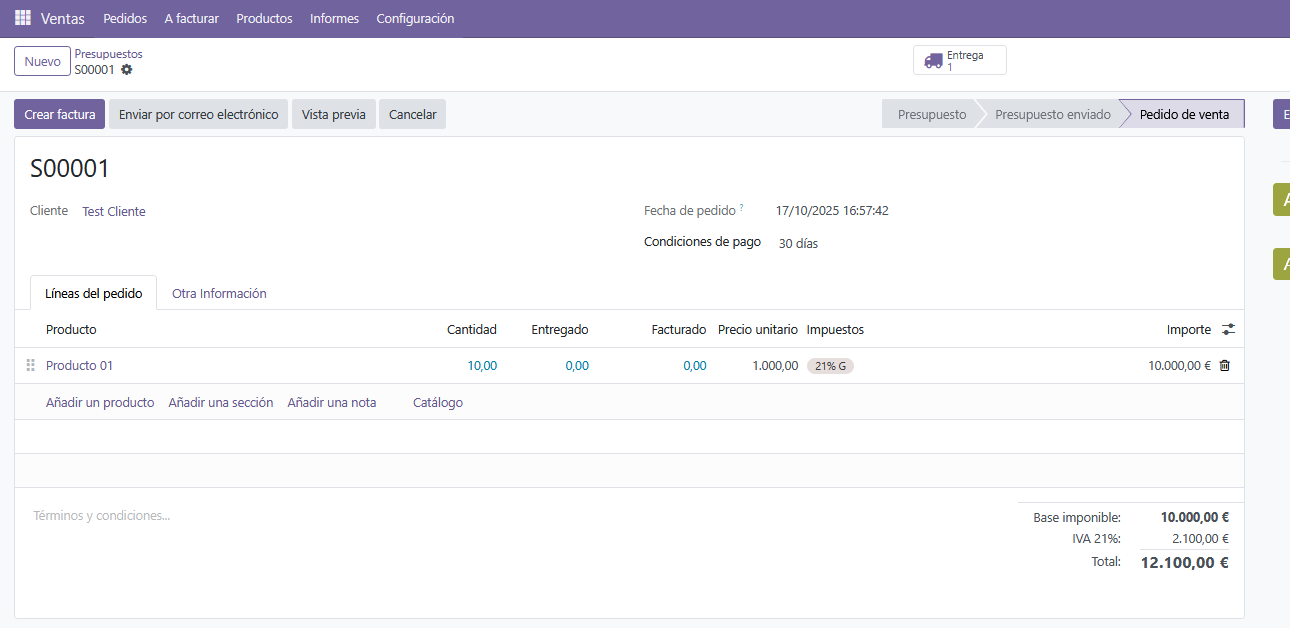
\includegraphics[width=0.5\textwidth]{pr2odoo43-presupuestoCreado.png}
    \caption{Presupuesto creado}
\end{figure}
\FloatBarrier

\begin{figure}[h!]
    \centering
    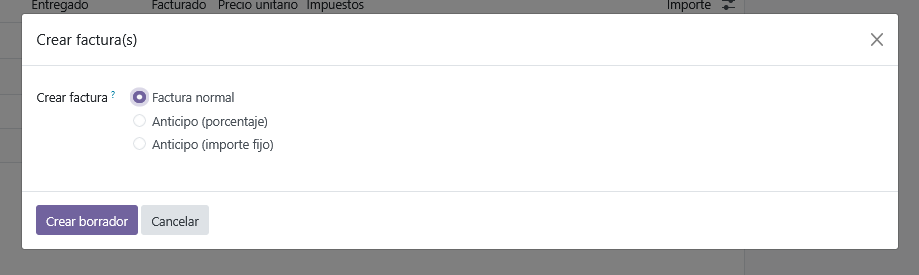
\includegraphics[width=0.5\textwidth]{pr2odoo44-crearBorradorFactura.png}
    \caption{Pantalla de creación de borrador de factura}
\end{figure}
\FloatBarrier

\begin{figure}[h!]
    \centering
    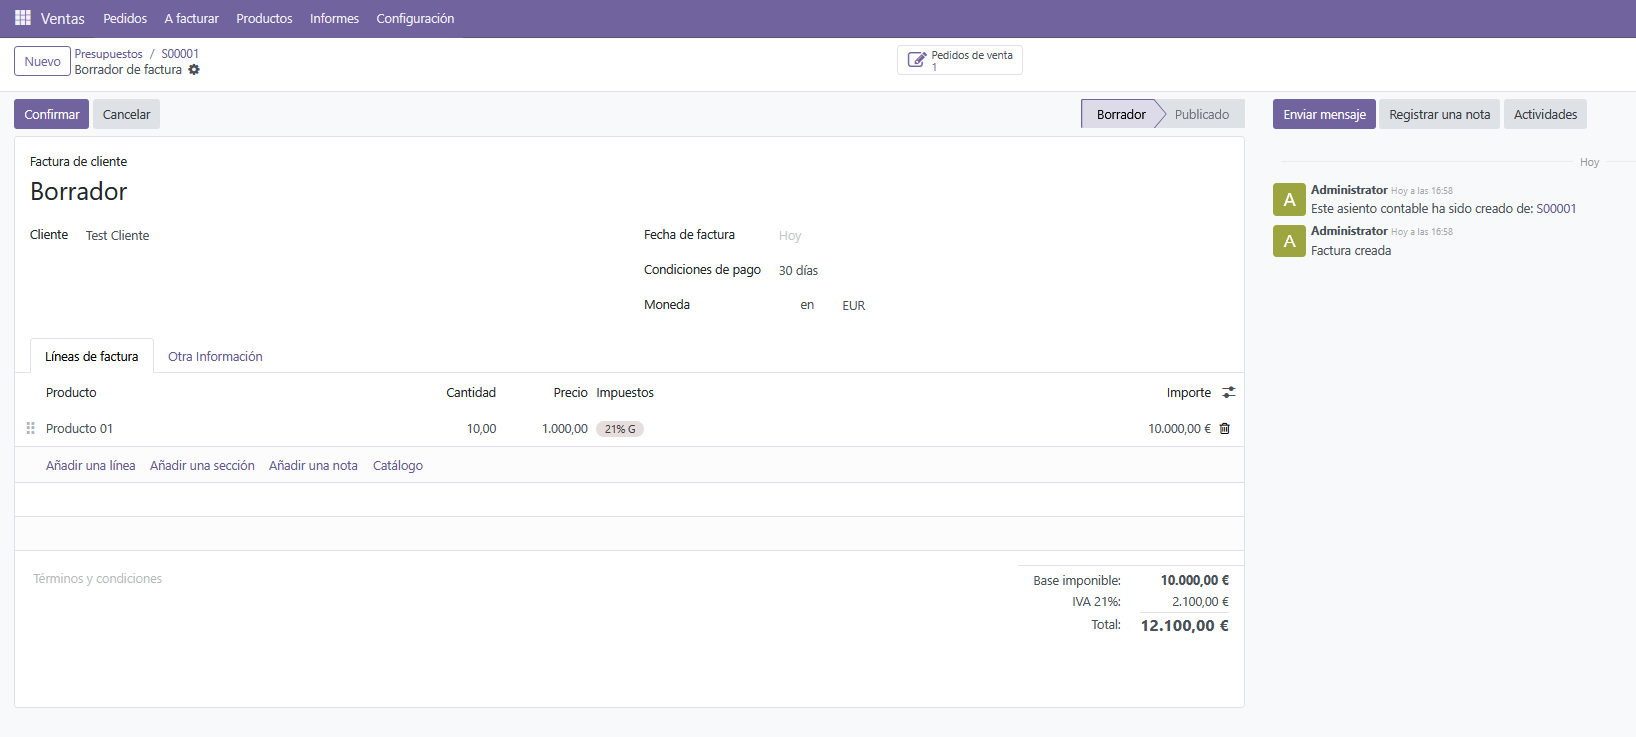
\includegraphics[width=0.5\textwidth]{pr2odoo45-borradorCreado.png}
    \caption{Borrador de factura creado}
\end{figure}
\FloatBarrier

\begin{figure}[h!]
    \centering
    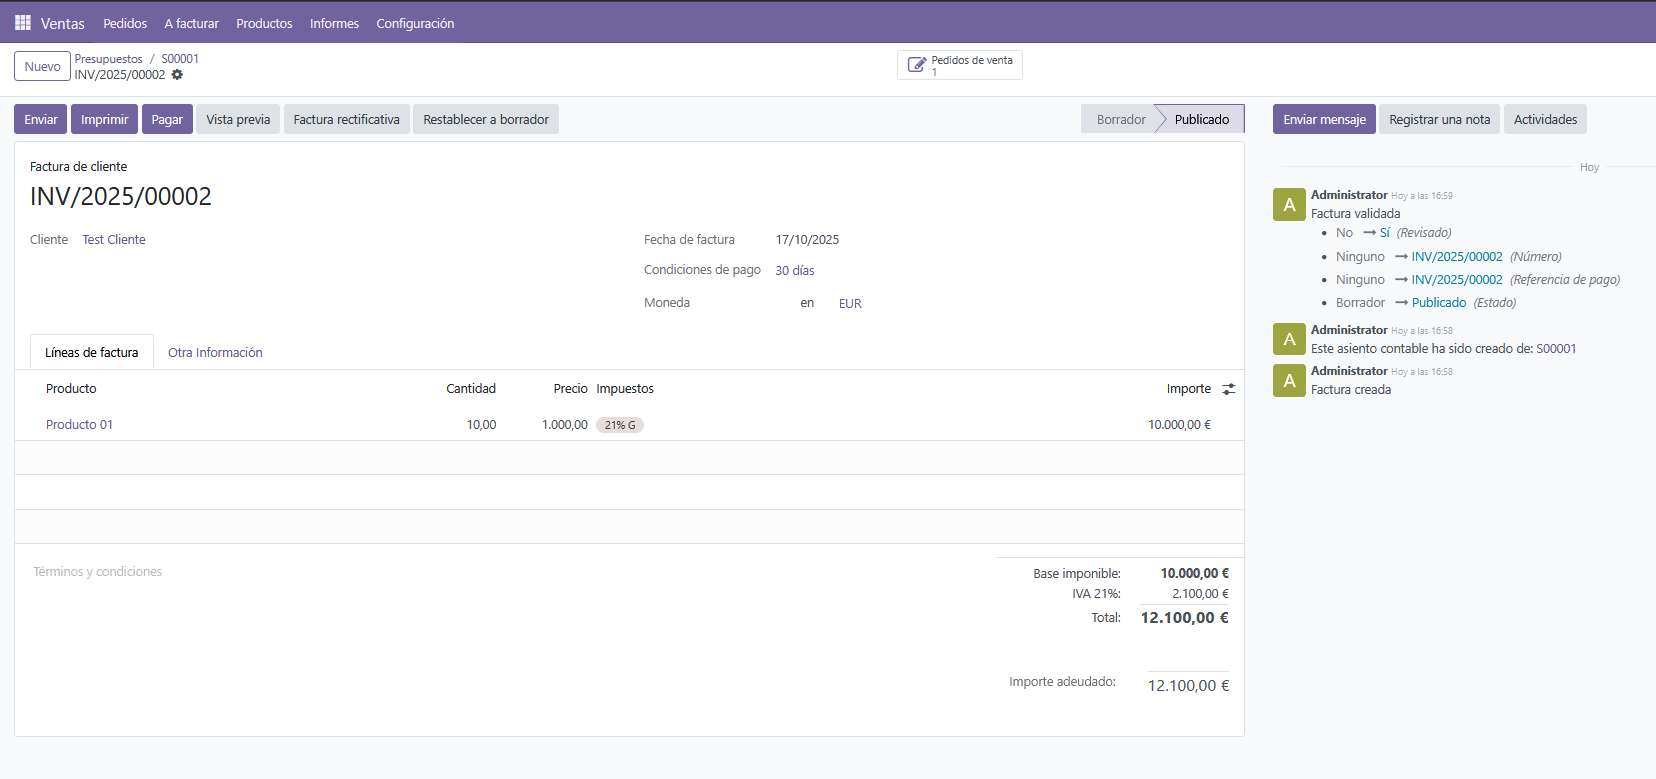
\includegraphics[width=0.5\textwidth]{pr2odoo46-facturaCreada.png}
    \caption{Factura creada}
\end{figure}
\FloatBarrier

\begin{figure}[h!]
    \centering
    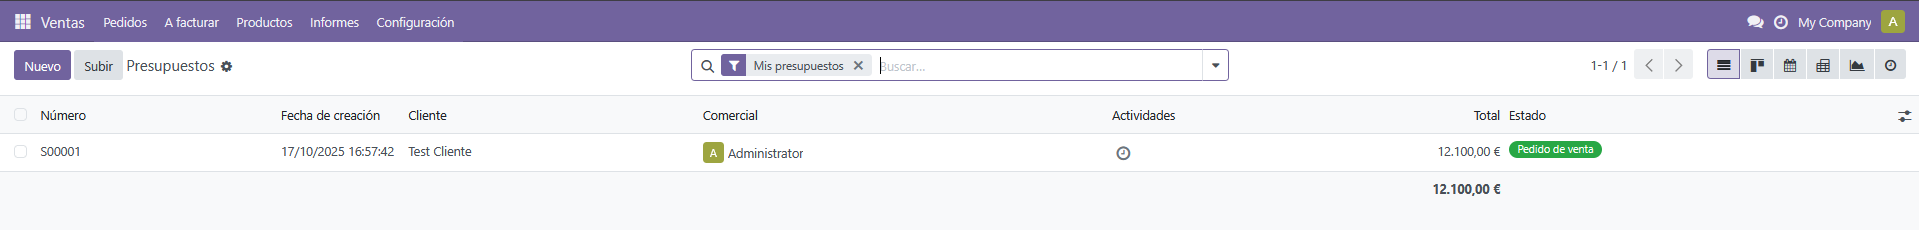
\includegraphics[width=0.5\textwidth]{pr2odoo47-listaVentas.png}
    \caption{Lista de ventas}
\end{figure}
\FloatBarrier

\subsection{Punto de venta}
\hyperlink{anchor-indice}{\textbf{Volver}}\\

\begin{figure}[h!]
    \centering
    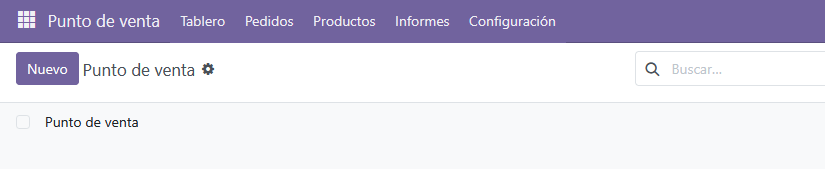
\includegraphics[width=0.5\textwidth]{pr2odoo48-pantallaPrincipal.png}
    \caption{Pantalla principal}
\end{figure}
\FloatBarrier

\begin{figure}[h!]
    \centering
    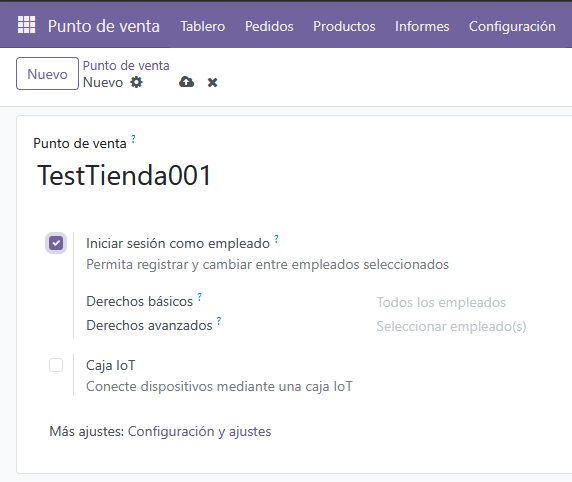
\includegraphics[width=0.5\textwidth]{pr2odoo49-nuevoTPV.png}
    \caption{Creación de punto de venta}
\end{figure}
\FloatBarrier

\begin{figure}[h!]
    \centering
    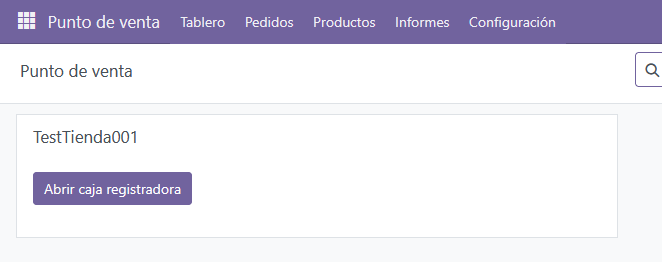
\includegraphics[width=0.5\textwidth]{pr2odoo50-tpvCreado.png}
    \caption{Punto de venta creado}
\end{figure}
\FloatBarrier

\begin{figure}[h!]
    \centering
    \includegraphics[width=0.5\textwidth]{pr2odoo51-modoAcceso.png}
    \caption{Modo de acceso (Usuario/PIN)}
\end{figure}
\FloatBarrier

\begin{figure}[h!]
    \centering
    \includegraphics[width=0.5\textwidth]{pr2odoo52-escojerCajero.png}
    \caption{Pantalla de seleccion de usuario}
\end{figure}
\FloatBarrier

\begin{figure}[h!]
    \centering
    \includegraphics[width=0.5\textwidth]{pr2odoo53-controlAperturaCaja.png}
    \caption{Pantalla de control de apertura de caja}
\end{figure}
\FloatBarrier

\begin{figure}[h!]
    \centering
    \includegraphics[width=0.5\textwidth]{pr2odoo54-creacionCliente.png}
    \caption{Creacion de nuevo cliente}
\end{figure}
\FloatBarrier

\begin{figure}[h!]
    \centering
    \includegraphics[width=0.5\textwidth]{pr2odoo55-clienteCreado.png}
    \caption{Cliente creado}
\end{figure}
\FloatBarrier

\begin{figure}[h!]
    \centering
    \includegraphics[width=0.5\textwidth]{pr2odoo56-operacionesCliente101.png}
    \caption{Operaciones con el cliente}
\end{figure}
\FloatBarrier

\begin{figure}[h!]
    \centering
    \includegraphics[width=0.5\textwidth]{pr2odoo57-diferentesClientesSimultaneos.png}
    \caption{Multiples clientes simultaneos}
\end{figure}
\FloatBarrier

\begin{figure}[h!]
    \centering
    \includegraphics[width=0.5\textwidth]{pr2odoo58-validacionPago.png}
    \caption{Validacion de pago}
\end{figure}
\FloatBarrier

\begin{figure}[h!]
    \centering
    \includegraphics[width=0.5\textwidth]{pr2odoo59-pagoCompletado101.png}
    \caption{Pago completado}
\end{figure}
\FloatBarrier

\begin{figure}[h!]
    \centering
    \includegraphics[width=0.5\textwidth]{pr2odoo60-cierreCaja.png}
    \caption{Cierre de caja}
\end{figure}
\FloatBarrier

\begin{figure}[h!]
    \centering
    \includegraphics[width=0.5\textwidth]{pr2odoo61-estadoFinalSesion.png}
    \caption{Estado final de sesión}
\end{figure}
\FloatBarrier

Cabe destacar que para crear categorias de productos, se puede crear desde el menu de Puntos de venta, y desde la pestaña "Puntos de Venta" de cada producto, asignarle la categoria que le corresponda.

Las pestañas de configuración permiten:
\begin{itemize}
    \item Tablero - Ver todas las tiendas creadas.
    \item Pedidos:
    \begin{itemize}
        \item  Pedidos.
        \item  Sesiones.
        \item  Pagos.
        \item  Clientes.
    \end{itemize}
    \item Productos - variantes y combinaciones.
    \item Informes de ventas, pedidos y de sesión.
    \item Configuración:
    \begin{itemize}
        \item  Ajustes de pago.
        \item  Terminal TPV.
        \item  Categorías de producto y atributos.
    \end{itemize}
\end{itemize}


\subsection{Contactos}
\hyperlink{anchor-indice}{\textbf{Volver}}\\

Es un módulo muy sencillo, recoje en un mismo sitio todos los contactos existentes en la base de datos. Permite no solo ver sino también modificar, añadir, eliminar, mandar comunicaciones, etc.

\begin{figure}[h!]
    \centering
    \includegraphics[width=0.5\textwidth]{pr2odoo62-pantallaPrincipal.png}
    \caption{Pantalla principal}
\end{figure}
\FloatBarrier

\begin{figure}[h!]
    \centering
    \includegraphics[width=0.5\textwidth]{pr2odoo63-edicionContacto.png}
    \caption{Edición de contacto}
\end{figure}
\FloatBarrier


\begin{figure}[h!]
    \centering
    \includegraphics[width=0.5\textwidth]{pr2odoo64-nuevoContacto.png}
    \caption{Nuevo contacto}
\end{figure}
\FloatBarrier


\begin{figure}[h!]
    \centering
    \includegraphics[width=0.5\textwidth]{pr2odoo65-opcionesContacto.png}
    \caption{Opciones de contacto}
\end{figure}
\FloatBarrier

\subsection{CRM}
\hyperlink{anchor-indice}{\textbf{Volver}}\\

CRM (Customer Relationship Management) es un pequeño pero curioso modulo que permite controlar el estado de oportunidades (negociaciones, tratos, etc). Es básicamente un tablero Kanban.

\begin{figure}[h!]
    \centering
    \includegraphics[width=0.5\textwidth]{pr2odoo66-pantallaPrincipal.png}
    \caption{Pantalla principal}
\end{figure}
\FloatBarrier

\begin{figure}[h!]
    \centering
    \includegraphics[width=0.5\textwidth]{pr2odoo67-nuevaOportunidad.png}
    \caption{Nueva oportunidad}
\end{figure}
\FloatBarrier

\begin{figure}[h!]
    \centering
    \includegraphics[width=0.5\textwidth]{pr2odoo68-oportunidadCreada.png}
    \caption{Oportunidad creada}
\end{figure}
\FloatBarrier

\begin{figure}[h!]
    \centering
    \includegraphics[width=0.5\textwidth]{pr2odoo69-oportunidadOpciones.png}
    \caption{Opciones de oportunidad}
\end{figure}
\FloatBarrier

\begin{figure}[h!]
    \centering
    \includegraphics[width=0.5\textwidth]{pr2odoo70-oportunidadGanado.png}
    \caption{Cambio de estado: Ganado}
\end{figure}
\FloatBarrier

\begin{figure}[h!]
    \centering
    \includegraphics[width=0.5\textwidth]{pr2odoo71-oportunidadPerdida.png}
    \caption{Cambio de estado: Pantalla de Perdido}
\end{figure}
\FloatBarrier

\begin{figure}[h!]
    \centering
    \includegraphics[width=0.5\textwidth]{pr2odoo72-cambioDeEtapa.png}
    \caption{}
\end{figure}
\FloatBarrier

\begin{figure}[h!]
    \centering
    \includegraphics[width=0.5\textwidth]{pr2odoo72-cambioDeEtapa.png}
    \caption{Cambio de etapa desde interfaz de opciones}
\end{figure}
\FloatBarrier

\begin{figure}[h!]
    \centering
    \includegraphics[width=0.5\textwidth]{pr2odoo73-añadirOportunidadDirectamenteEnEtapa.png}
    \caption{Creacion de oportunidad directamente en la etapa deseada}
\end{figure}
\FloatBarrier

\begin{figure}[h!]
    \centering
    \includegraphics[width=0.5\textwidth]{pr2odoo74-crearEtapa.png}
    \caption{Creación de etapa}
\end{figure}
\FloatBarrier

\begin{figure}[h!]
    \centering
    \includegraphics[width=0.5\textwidth]{pr2odoo75-cambioManualDeEtapa.png}
    \caption{Cambio manual de etapa (en este caso, a Ganado)}
\end{figure}
\FloatBarrier

En la pestaña de Ventas se puede no solo ver el flujo actual, sino también generar nuevas actividades, ver y editar presupuestos, equipos y clientes.

Informes abarca las secciones de pronóstico, flujo, leads y actividades.

Configuración permite editar:
\begin{enumerate}
    \item Equipos de ventas
    \item Actividades:
    \begin{enumerate}
        \item Tipos.
        \item Planes.
    \end{enumerate}
    \item flujo
    \begin{enumerate}
        \item Etiquetas
        \item Razones de pérdida
    \end{enumerate}
    \item Generación de leads: Solicitudes de minería.
\end{enumerate}

\section{Copias de seguridad}
\hyperlink{anchor-indice}{\textbf{Volver}}\\

\subsection{Base de datos}

\subsubsection{Interfaz}
\hyperlink{anchor-indice}{\textbf{Volver}}\\

Dirección en navegador para realizar backup:
\begin{verbatim}
    http://localhost:9001/web/database/manager
\end{verbatim}


\begin{figure}[h!]
    \centering
    \includegraphics[width=0.5\textwidth]{pr2odoo76-backupInterfazPrincipal.png}
    \caption{Pantalla principal}
\end{figure}
\FloatBarrier

\begin{figure}[h!]
    \centering
    \includegraphics[width=0.5\textwidth]{pr2odoo77-backupInterfazPantallaCambio.png}
    \caption{Pantalla de backup}
\end{figure}
\FloatBarrier

\begin{figure}[h!]
    \centering
    \includegraphics[width=0.5\textwidth]{pr2odoo78-backupInterfazDescargado.png}
    \caption{Backup descargado}
\end{figure}
\FloatBarrier

\subsubsection{Comandos}
\hyperlink{anchor-indice}{\textbf{Volver}}\\

Comando: 
\begin{verbatim}
    docker ps
\end{verbatim}

\begin{figure}[h!]
    \centering
    \includegraphics[width=0.5\textwidth]{pr2odoo79-dockerPS.png}
    \caption{Información de los contenedores}
\end{figure}
\FloatBarrier

Comando: 
\begin{verbatim}
    docker exec 98832932c559 pg_dump -U odoo -F c odoo_test > C:\odoo_backups\odoo_backup.sql 
\end{verbatim}

\begin{itemize}
    \item 98832932c559: ID del contenedor
    \item odoo\_test: nombre de la base de datos
    \item C:/odoo\_backups/odoo\_backup.sql: ruta donde guardaremos la copia de seguridad
\end{itemize}

\begin{figure}[h!]
    \centering
    \includegraphics[width=0.5\textwidth]{pr2odoo80-comandoBackup.png}
    \caption{Comando para realizar backup}
\end{figure}
\FloatBarrier

\begin{figure}[h!]
    \centering
    \includegraphics[width=0.5\textwidth]{pr2odoo81-backupRealizado.png}
    \caption{Backup realizado}
\end{figure}
\FloatBarrier

\subsection{Archivo de configuración de Odoo}
\hyperlink{anchor-indice}{\textbf{Volver}}\\

Comando: 
\begin{verbatim}
    docker exec -it e0.bigodoo.net mkdir -p /etc/odoo
\end{verbatim}

\begin{itemize}
    \item e0.bigodoo.net: nombre del contenedor (el ID también es válido)
    \item /etc/odoo: directorio a crear
\end{itemize}

\begin{figure}[h!]
    \centering
    \includegraphics[width=0.5\textwidth]{pr2odoo82-crearDirectorio.png}
    \caption{Crear directorio de archivo de configuración}
\end{figure}
\FloatBarrier

Comando: 
\begin{verbatim}
    docker exec -it e0.bigodoo.net cp /etc/odoo/odoo.conf /etc/odoo/odoo.conf.backup
\end{verbatim}

\begin{itemize}
    \item e0.bigodoo.net: nombre del contenedor (el ID también es válido)
    \item /etc/odoo/odoo.conf: archivo a copiar
    \item /etc/odoo/odoo.conf.backup: ruta para la copia
\end{itemize}

\begin{figure}[h!]
    \centering
    \includegraphics[width=0.5\textwidth]{pr2odoo83-crearBackup.png}
    \caption{Crear archivo de backup}
\end{figure}
\FloatBarrier

Comando: 
\begin{verbatim}
    docker exec -it e0.bigodoo.net ls -la /etc/odoo/odoo.conf.backup
\end{verbatim}

\begin{itemize}
    \item e0.bigodoo.net: nombre del contenedor (el ID también es válido)
    \item /etc/odoo/odoo.conf.backup: archivo a comprobar
\end{itemize}

\begin{figure}[h!]
    \centering
    \includegraphics[width=0.5\textwidth]{pr2odoo84-comprobarBackup.png}
    \caption{Comprobar existencia de backup}
\end{figure}
\FloatBarrier

Comando: 
\begin{verbatim}
    docker cp e0.bigodoo.net:/etc/odoo/odoo.conf.backup C:/odoobackup
\end{verbatim}

\begin{itemize}
    \item e0.bigodoo.net: nombre del contenedor (el ID también es válido)
    \item /etc/odoo/odoo.conf.backup: archivo a copiar
    \item /etc/odoo/odoo.conf.backup: ruta para la copia en host
\end{itemize}

\begin{figure}[h!]
    \centering
    \includegraphics[width=0.5\textwidth]{pr2odoo85-copiarBackupAhost.png}
    \caption{Copiar archivo de backup a host}
\end{figure}
\FloatBarrier

\begin{figure}[h!]
    \centering
    \includegraphics[width=0.5\textwidth]{pr2odoo86-backupCopiado.png}
    \caption{Backup copiado a host}
\end{figure}
\FloatBarrier
\end{document}
